\hypertarget{introduction}{%
\section{Introduction}\label{introduction2}}

The motivation of this thesis was twofold: firstly, to produce three-dimensional epithelia with controlled pressure, and secondly, to study the material response of the tissue to different regimes of tension. To achieve the first objective, we have developed a monolayer inflator (MOLI) device that allows us to create epithelial domes where cells can be stretched to more than 100\% of areal strain.

Epithelial tissue plays a crucial role in various physiological functions, and must therefore undergo deformation over a wide range of timescales and magnitudes. Similarly, pressure levels also vary widely in different contexts \cite{torres-sanchez2021, choudhury2022a}. For instance, the luminal pressure in blastocysts doubles over the course of its development, resulting in changes in cortical tension and strain \cite{chan2019}. The MDCK dome system provides a suitable platform to investigate the interplay between cell strain, tension, and pressure. Previous studies by Latorre et al. have observed a wide range of pressure throughout the evolution of the dome, and cells have exhibited a range of deformation, including active-superelastic behavior \cite{latorre2018}. However, the control in this system is limited to the footprint of the domes. In this chapter, we aim to utilize the MOLI system to subject tissues to a range of strain and tension regimes.

\hypertarget{measurement-of-dome-mechanics}{%
	\section{Measurement of dome
		mechanics}\label{measurement-of-dome-mechanics}}


To measure the kinematics of the domes, we analyzed the midsection of the domes, assuming symmetry of spherical caps (see fig \ref{fig_7_1}). We measured the height ($h$) and base radius ($a$). This allowed us to calculate the radius of curvature ($R$) using trigonometry as 
$$ R = \frac{h^2 + a^2}{2h}.$$ 
The measurement of pressure ($\Delta P$) allowed us to compute the tension ($\sigma$), given by Laplace's law 
$$\sigma = \frac{\Delta PR }{2} .$$
For the dome strain, we used the areal strain measure, which is computed based on the surface area. We compared the dome surface area ($A$) to the area of the footprint ($A_{0}$).
$$ \epsilon = \frac{A - A_{0}}{A_{0}} = \frac{\pi(h^2 + a^2) - \pi a^2}{\pi a^2} = \frac{h^2}{a^2} .$$
By utilizing the line scanning modality of a Zeiss Airy Scan Microscope, we were able to quickly obtain a significant number of frames for the analysis of height and radius of curvature of the domes. To this end, we generated kymographs by creating cross-sectional images of the top section of the domes with respect to time. The kymographs were processed using MATLAB-based image analysis code to determine the time evolution of the dome height and base radius. Specifically, the location of the maximum intensity value for a given time point in the graph was used to track the time-dependent height of the dome, while the same approach was utilized to obtain the time-dependent base radius. Importantly, he kymograph of the base radius allowed us to keep track of delamination, as it could change the value of strain.

\begin{figure}
	\begin{minipage}[c]{0.7\textwidth}
		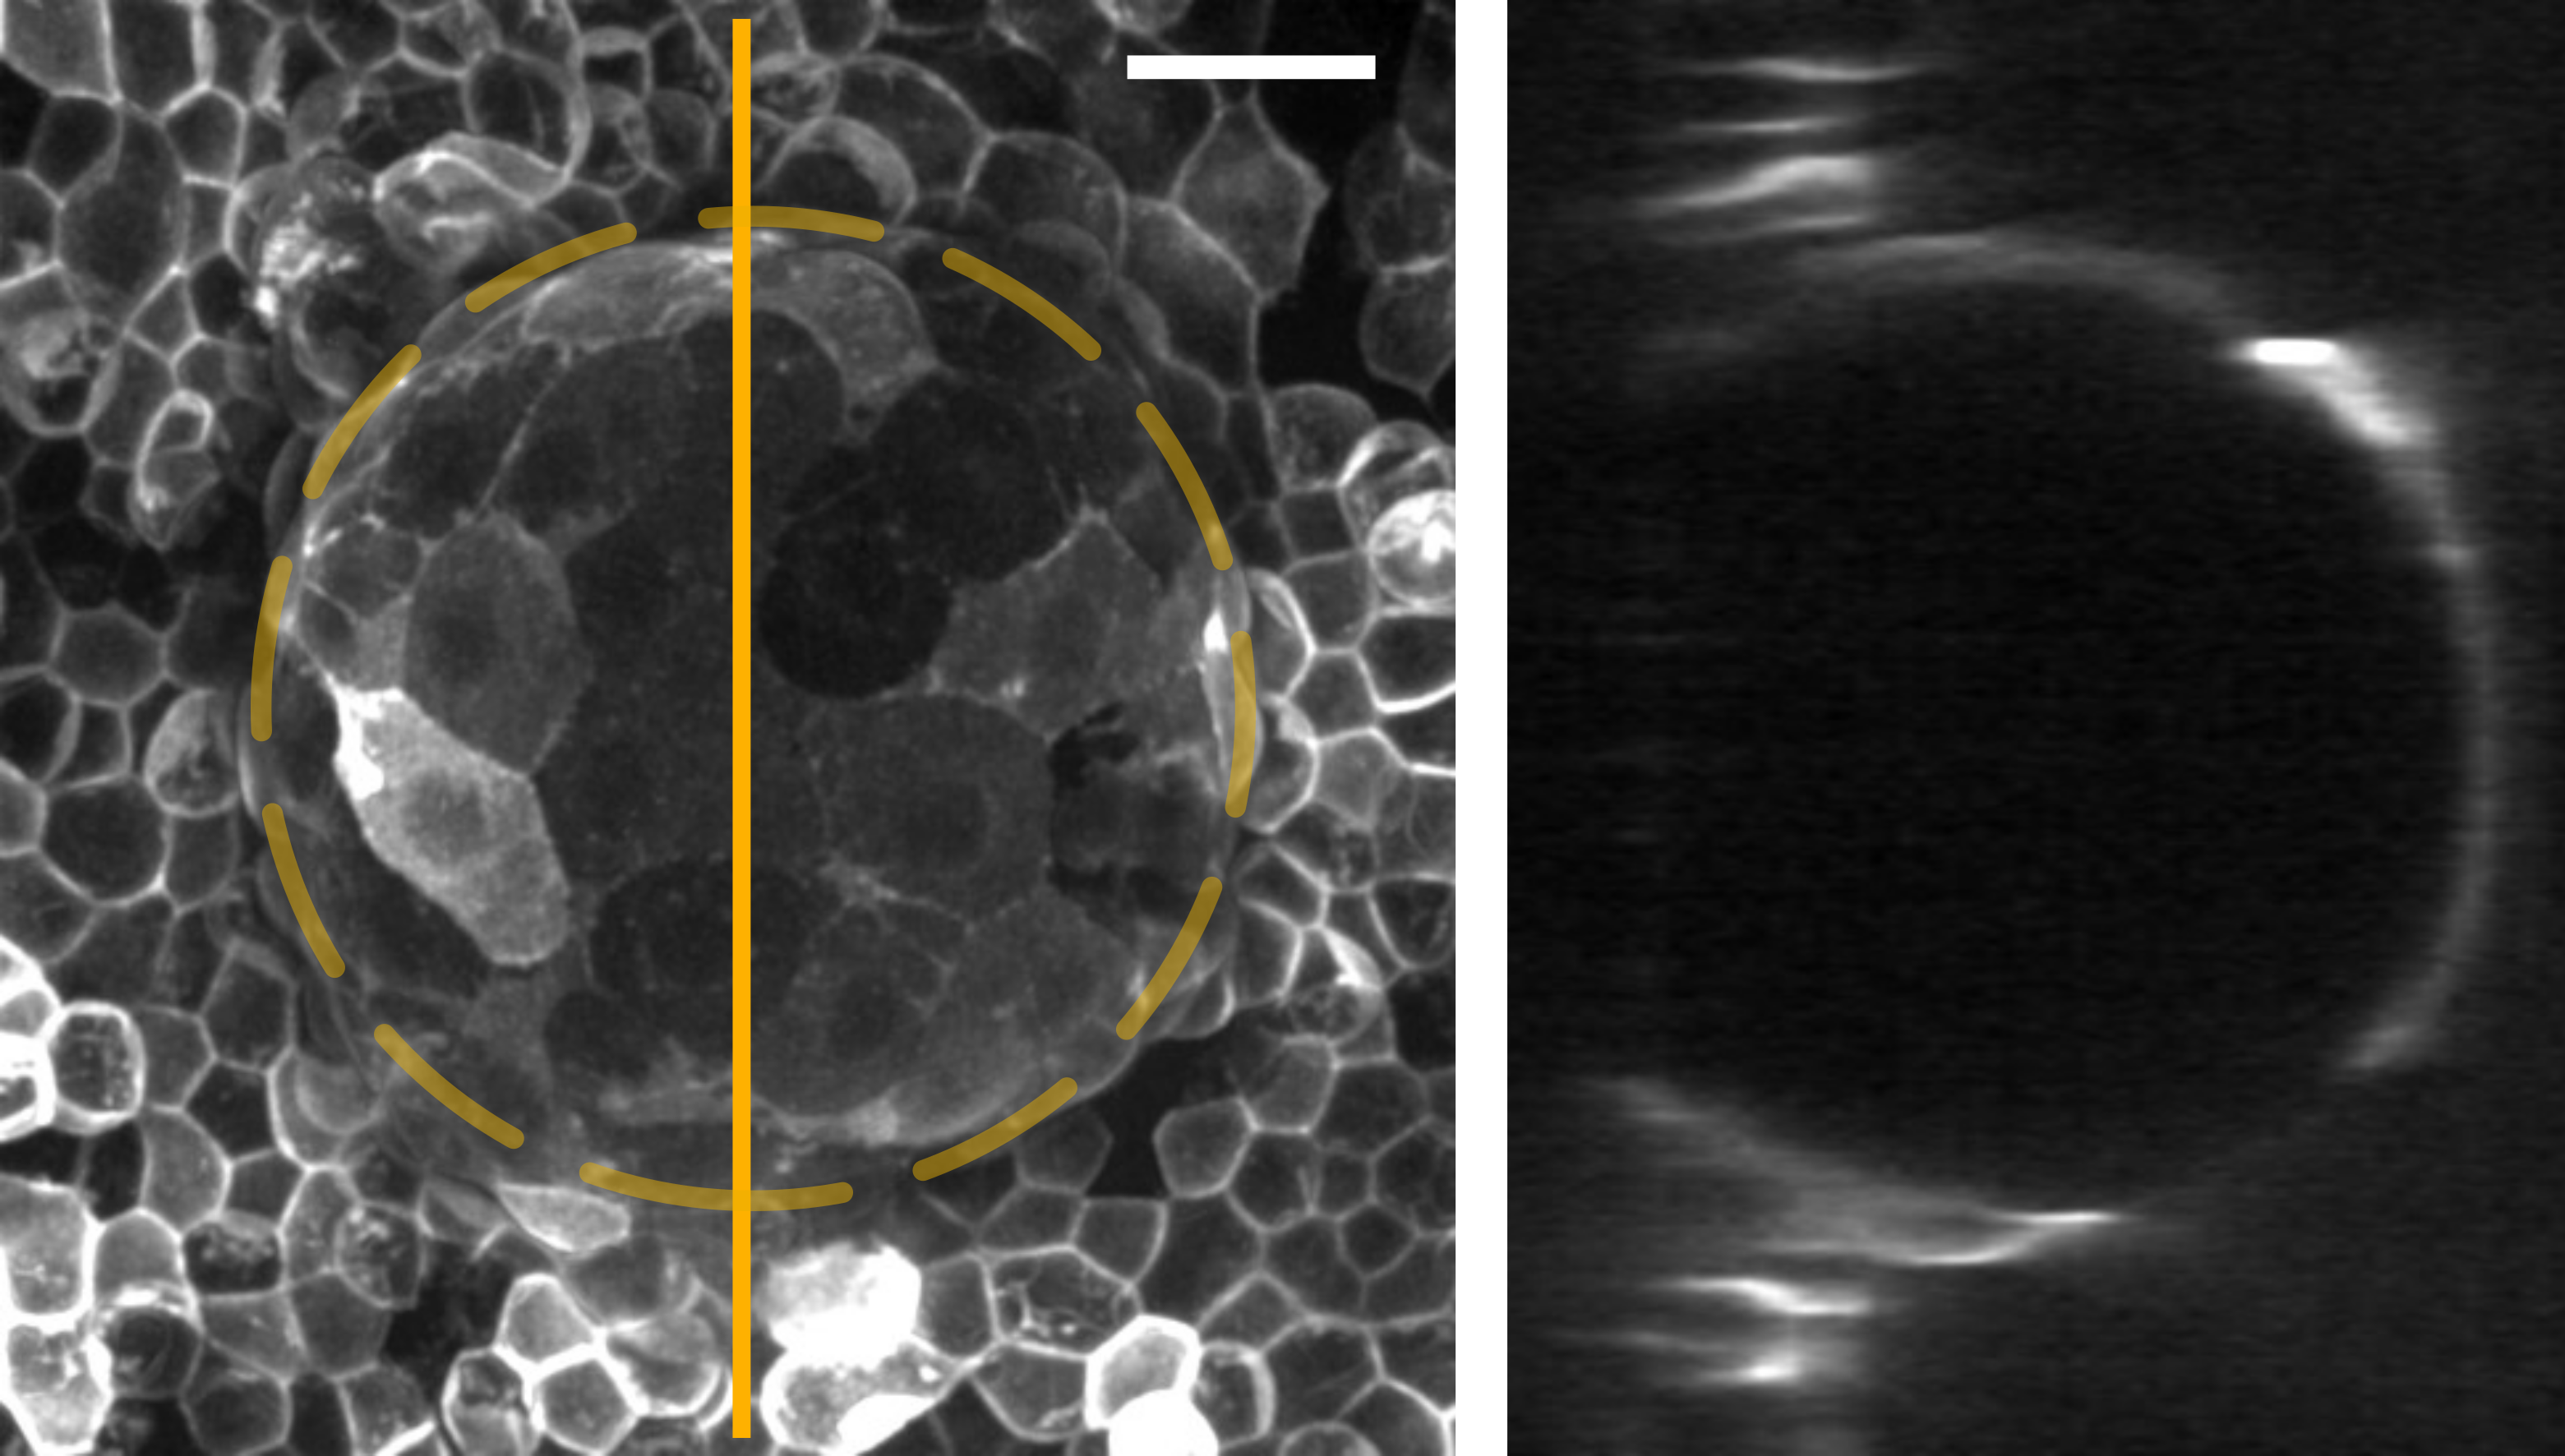
\includegraphics[width=\textwidth]{chap7_realdome.png}
	\end{minipage}\hfill
	\begin{minipage}[c]{0.27\textwidth}
		\caption{\\ \textbf{Spherical cap}:\\An example of an epithelial dome at 200 Pa, which has increased its surface area almost four times the original footprint. The spherical shape of the dome can be seen in the cross-section. Scale bar is  $20 \mu m$.
		} \label{fig_7_1}
	\end{minipage}
\end{figure}

\hypertarget{epithelial-domes-at-constant-pressure}{%
	\section{Epithelial domes at constant
		pressure}\label{epithelial-domes-at-constant-pressure}}

Initially, our focus was to investigate the behavior of domes under constant pressure. We systematically inflated domes at varying pressures ranging from 0-400\unit{\pascal}, but observed that hardly any of the domes formed at pressures lower than 50-100\unit{\pascal}, Thus, we settled on using 200\unit{\pascal} which allowed domes to form without delaminating out of pattern.

Our measurements show that the areal strain of the dome increases during the first three to five minutes of pressure application, and then reaches a plateau in strain until 5-10 minutes (see fig \ref{fig_7_3} A). Despite large dome-to-dome variability, with strains ranging from 50\% to 300\%, the stabilization in strain suggests that a steady state has been achieved by the tissue.

Upon further investigation of the tension-strain relationship exhibited by these domes, a distinct curve was observed, bearing resemblance to the swish symbol of "Nike" (see fig \ref{fig_7_3} B). The tension within the domes was found to be extremely high for low strains, followed by a decrease to a minimum value at an areal strain of one, where the dome assumes a perfect hemispherical shape. Subsequently, the tension increases once again, albeit with a slope that is comparably gentle in comparison to the steep decline observed at lower strains.

Such a material response is atypical for biaxially stretched materials. However, in this case, the underlying cause of the curve can be attributed to the geometric constraints imposed by the dome system and force balance, as governed by Laplace's law. Since the tension within the dome is intrinsically dependent on its radius of curvature, the initial high value of the radius of curvature leads to a correspondingly high tension that subsequently diminishes to a minimum upon assuming a hemispherical shape (see fig \ref{fig_7_4}). It is important to note that the radius of curvature, areal strain, and tension are all interconnected, such that the expression of the curve can be derived at a constant pressure. Given that radius of curvature and areal strain are

$$ R = \frac{h^2 + a^2}{2h}, \ \ \ \ \text{and} \ \ \ \ \epsilon = \frac{h^2}{a^2}.$$
By substituting areal strain ($\epsilon$) in the expression of radius of curvature ($R$),
$$ R = \frac{h^2/a^2 + 1}{2h/a^2} = a\frac{\epsilon + 1}{\sqrt{\epsilon}}.$$
By substituting ($R$) in Laplace’s law, we get the relation,
$$ \frac{\sigma}{a} = \frac{\Delta P}{4} \left( \frac{\epsilon + 1}{\sqrt{\epsilon}} \right).$$

Normalizing the tension with the base radius results in all domes collapsing onto one curve corresponding to a specific pressure. Thus, we could call these tension-strain curves "isobarics".

We recognize that when the step pressure is applied, the dome suddenly inflates and has to undergo non-steady state out-of-equilibrium stresses. It is clear that this curve does not represent the quasi-static constitutive relation of the epithelial tissue.

\begin{figure}[t]
	\centering
	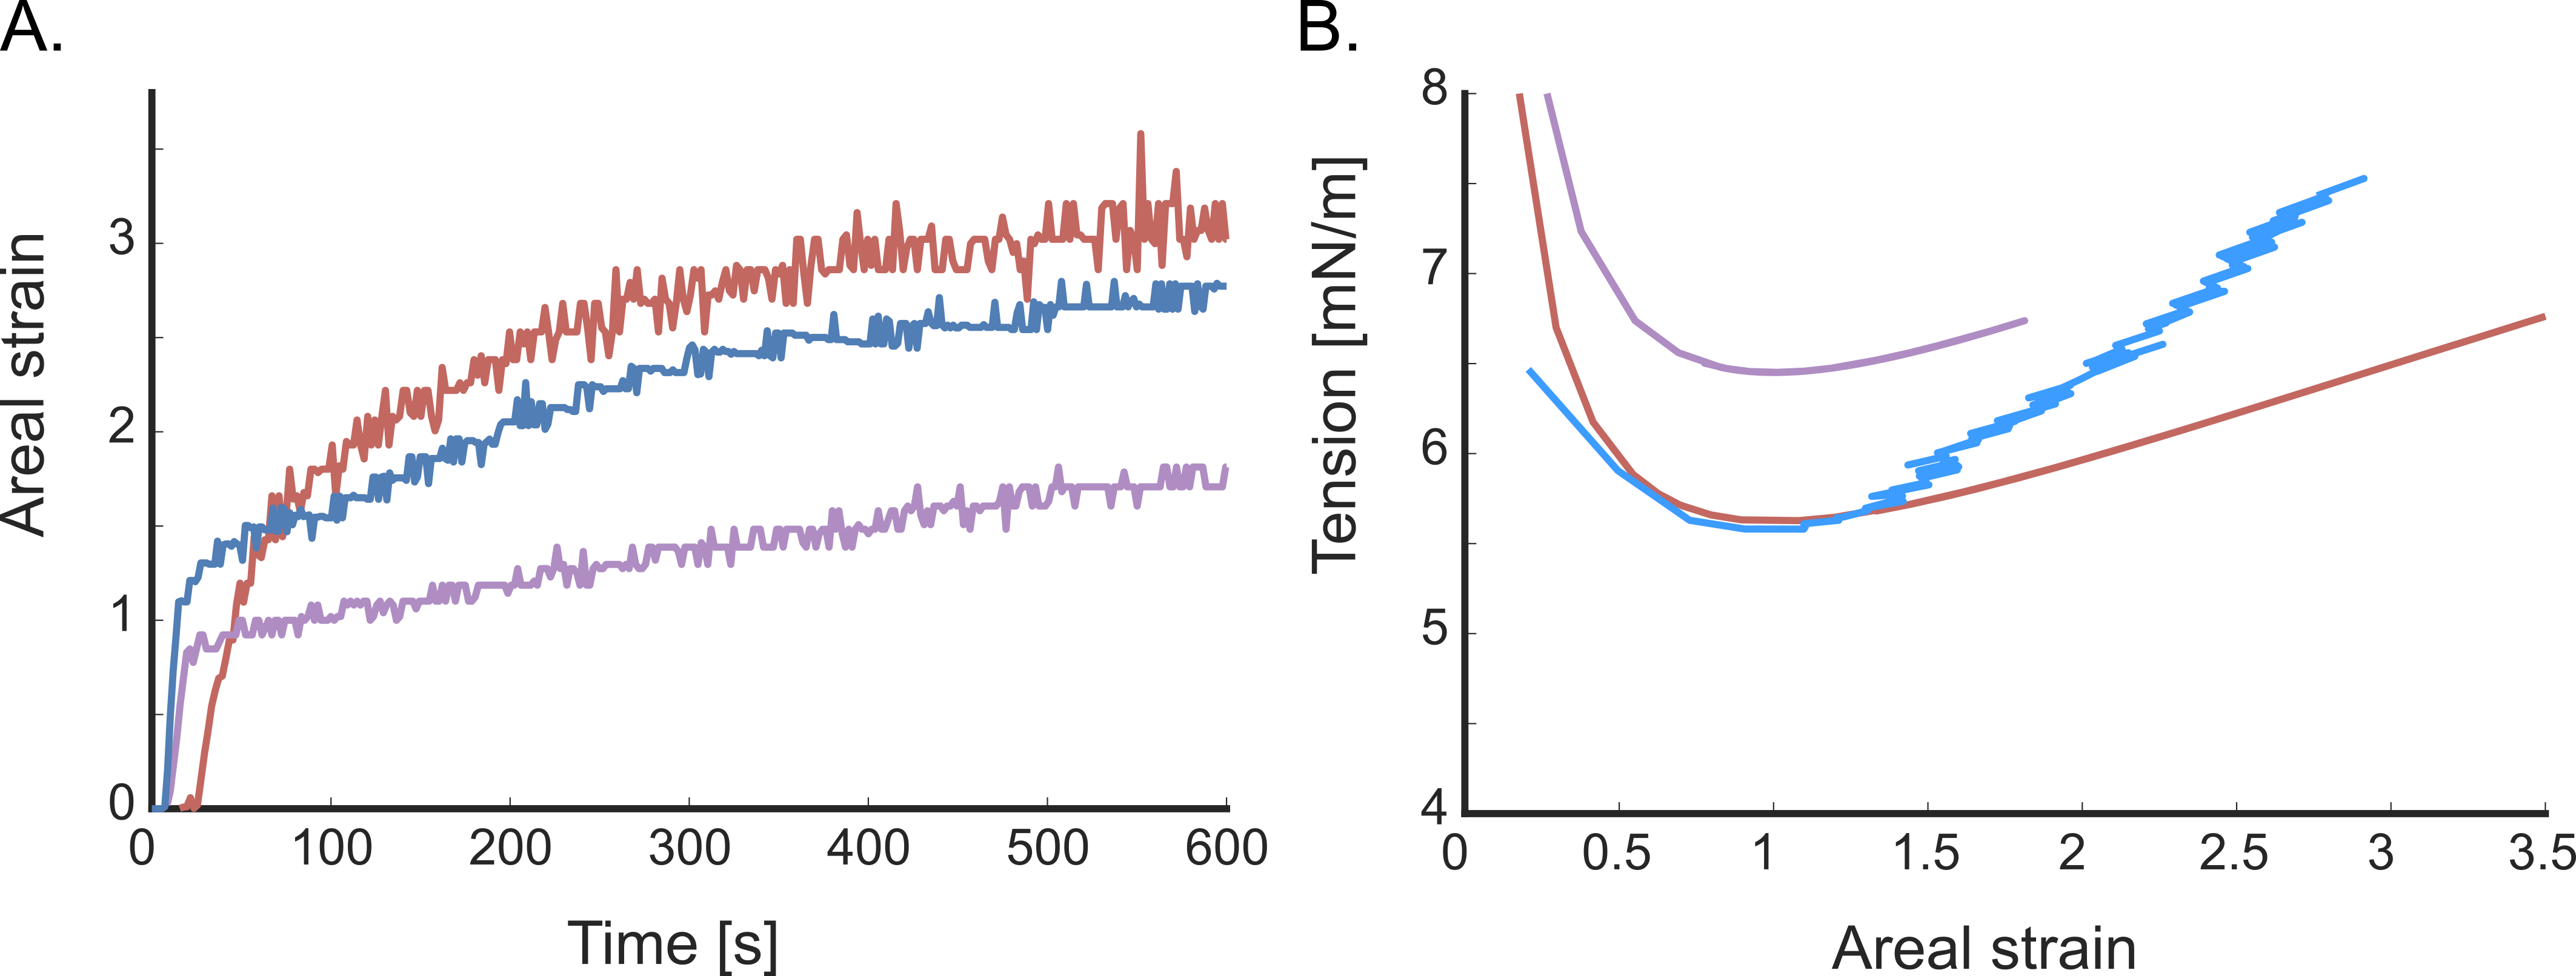
\includegraphics[width=\textwidth]{chap7_constpressure.png}
	\caption{\label{fig_7_3} \textbf{Epithelial domes at constant pressure}:Dynamic response of the representative domes at a constant pressure of 200 Pa: (A) Areal strain increases and reaches a steady state at around 5 minutes, and we can clearly see variability in the maximum strains. (B) The same domes produce a peculiar "NIKE swish" shaped tension and strain curve.
	}
\end{figure}

\begin{figure}
	\centering
	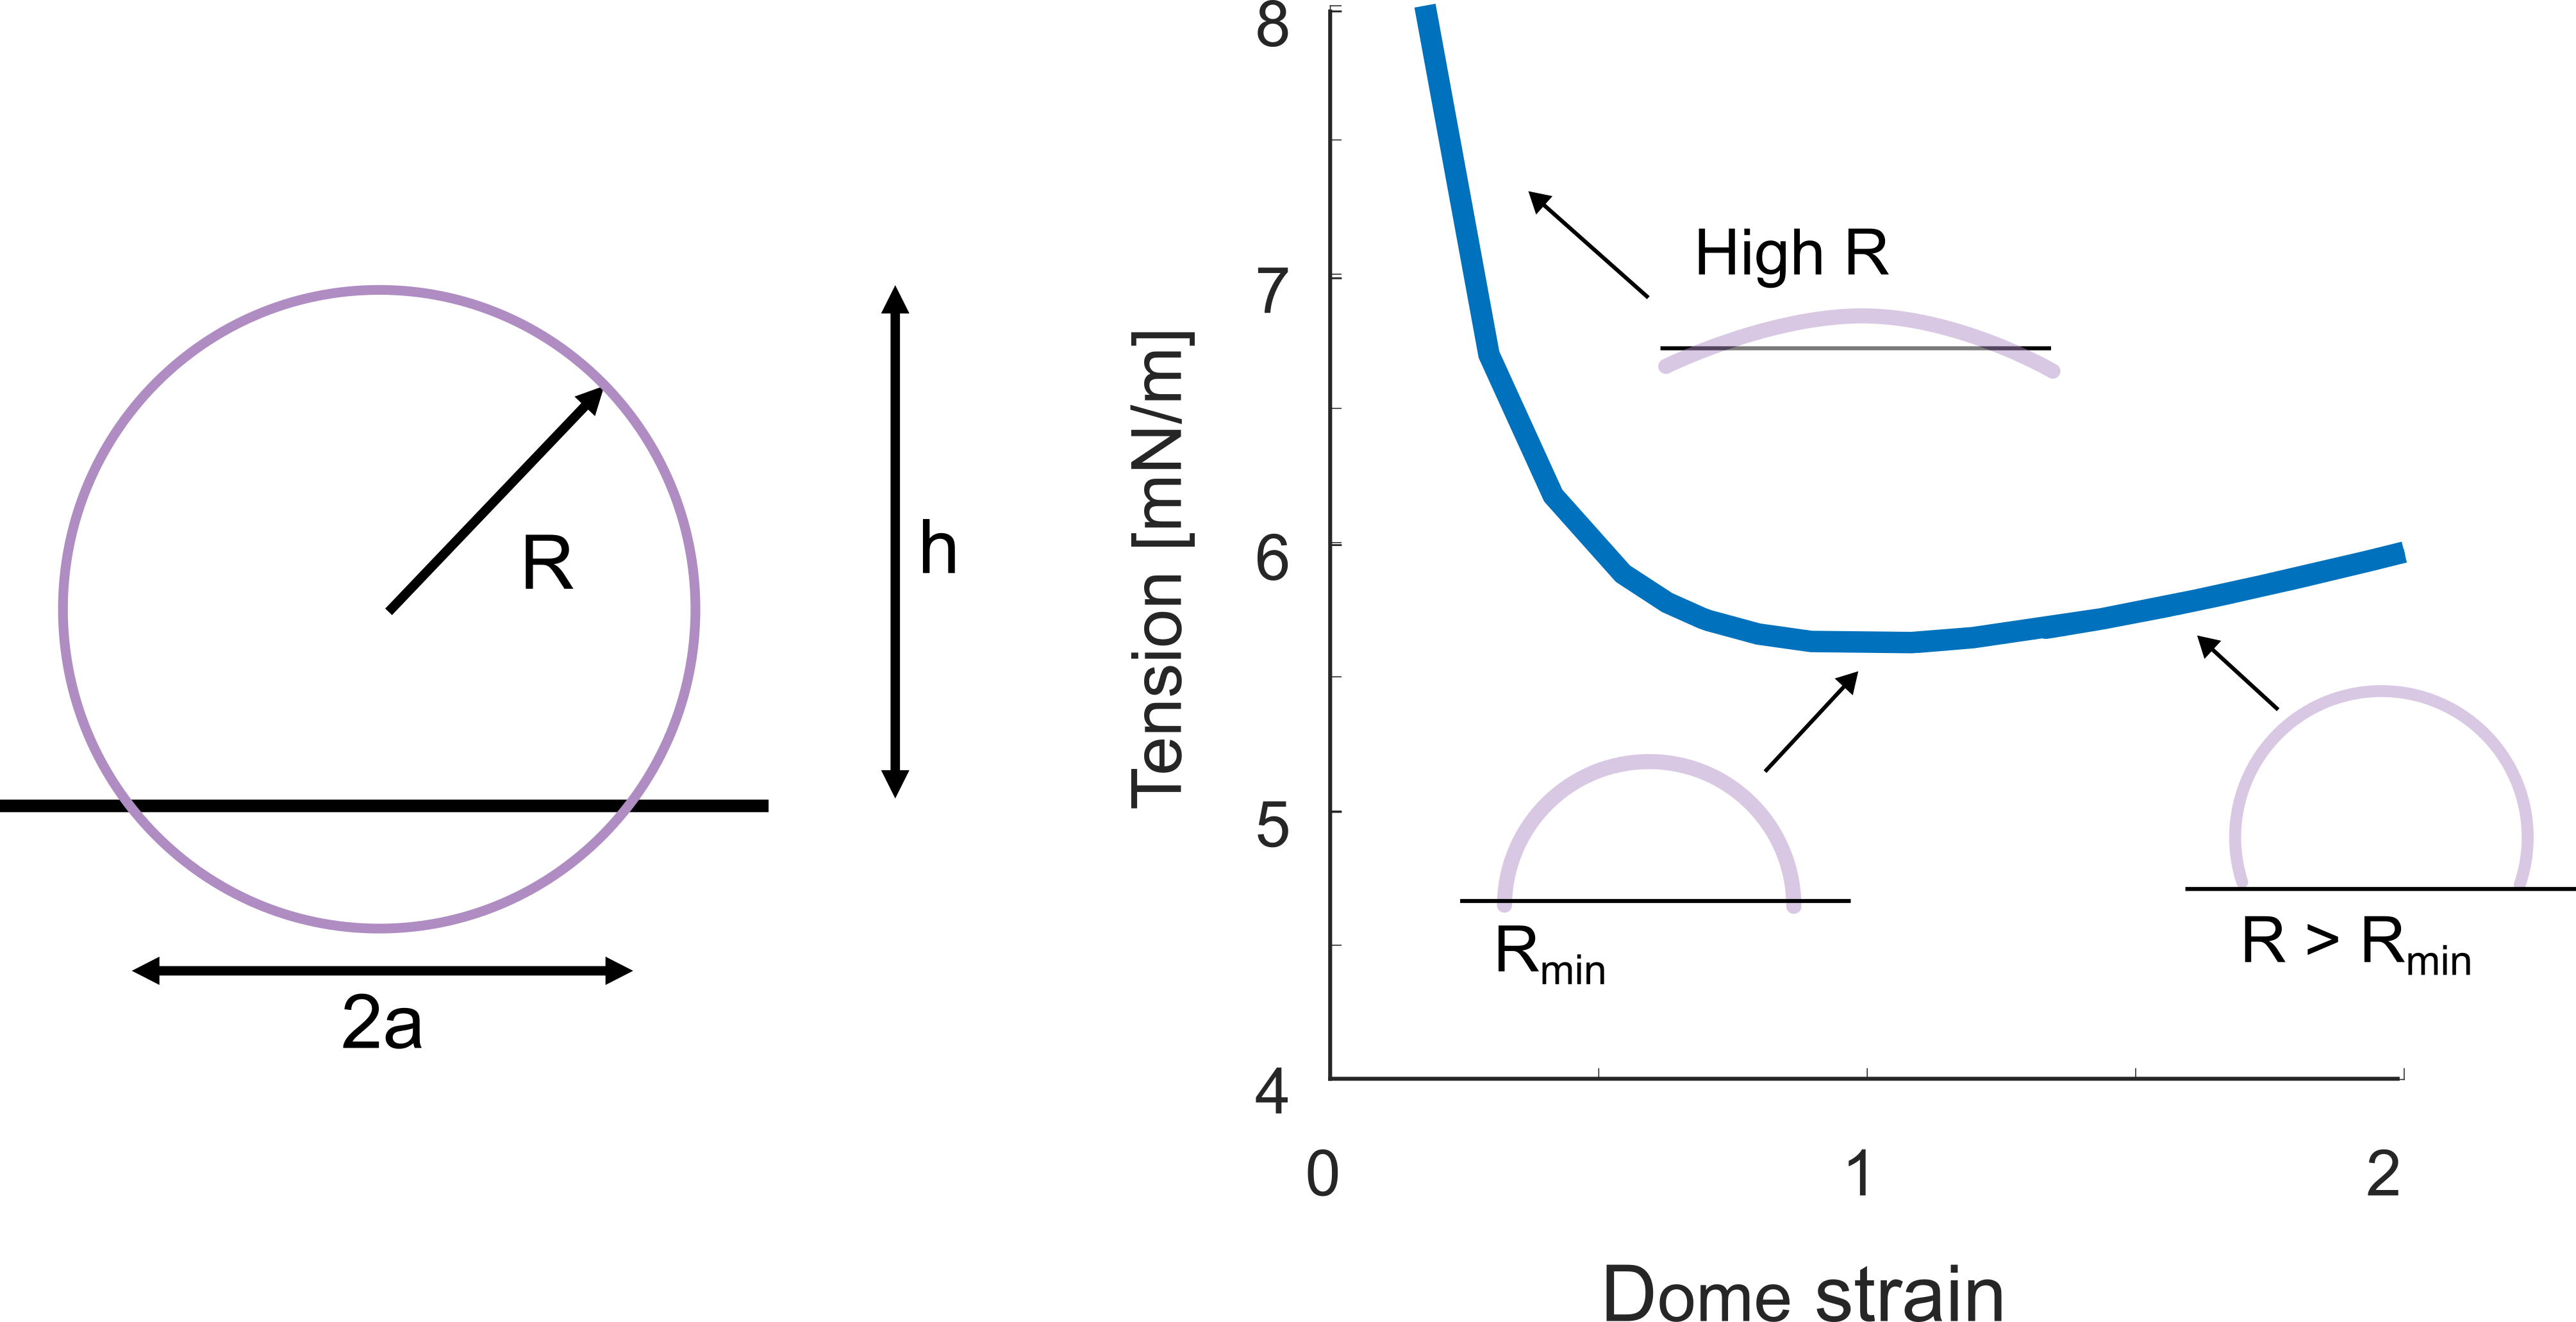
\includegraphics[width=0.8\textwidth]{chap7_radius.png}
	\caption{\label{fig_7_4} \textbf{Illustrative explanation for isobaric curve}: Tension and strain are related to each other through the geometric constraint of a spherical cap. Here, the base radius (a) is constant, so the radius of curvature is almost infinite for domes with very small strains (<0.05). As the strain increases, the radius of curvature decreases to a minimum corresponding to the base radius. Then it continues to increase again.	
	}
\end{figure}



\hypertarget{constitutive-relation-of-epithelia}{%
	\section{Constitutive relation of
		epithelia}\label{constitutive-relation-of-epithelia}}

In order to derive the actual constitutive relation of a material, it is preferable to apply strain or tension in a quasi-static manner. However, in our experimental system, only pressure could be controlled. Therefore, we employed pressure control to establish steady state tension across a range of strains. Slowly increasing pressure was not a practical approach for domes, as they do not delaminate at low pressures. In the case where delamination did occur, the domes would rapidly inflate, thus reaching steady state at higher strains. Consequently, steady state tensions at lower strains would not be accessible. To overcome this limitation, we devised experiments to capture the steady state of the domes by deflating them.

Specifically, we applied a pressure of 200 Pa for 5 minutes until the dome reached steady state. Subsequently, we reduced the pressure in increments of 20 Pa and allowed the dome to reach steady state at each step (see fig \ref{fig_7_5} A). This process was repeated until the dome was completely deflated. In this way, we were able to capture tension-strain curves at different isobarics as the dome passed through various states.

Ultimately, we obtained a constitutive relation that exhibits an initial increase in tension with strain for lower strains. However, for larger strains, the tension appears to plateau consistent with earlier studies on MDCK domes (see fig \ref{fig_7_5} B).It is worth noting that the variability in dome-to-dome tension is significant, and the tensions recorded around 4.5 \unit{mN/m} are of the same order of magnitude as those reported in previous studies \cite{latorre2018, marin-llaurado2022}.

\begin{figure}
	\centering
	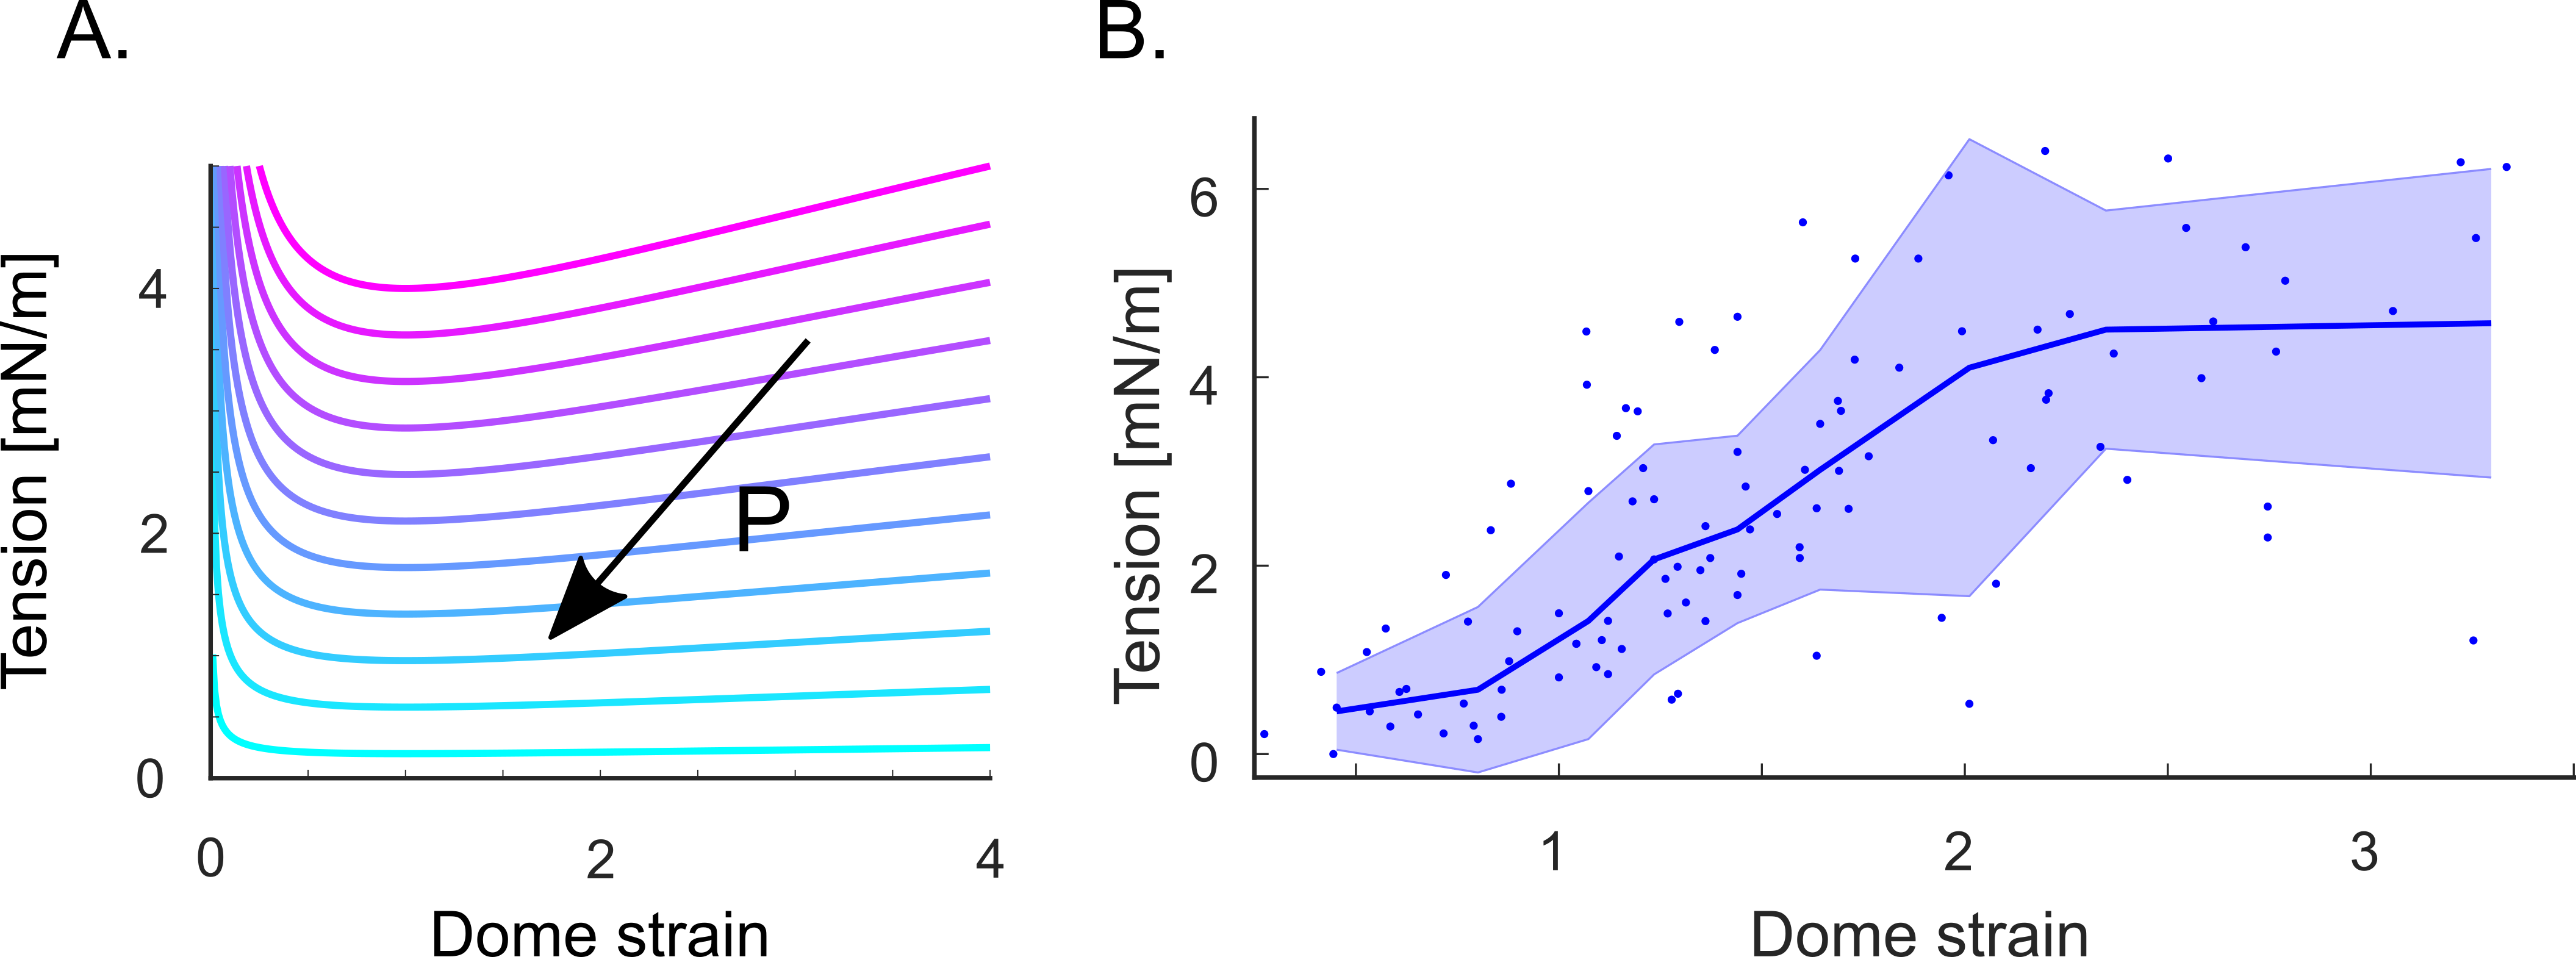
\includegraphics[width=\textwidth]{chap7_constitutivelaw.png}
	\caption{\label{fig_7_5} \textbf{Constitutive Relation of Epithelia}: (A) We will set up experiments to probe the steady state at different pressures. We will start from the highest pressure, move along the isobaric line and achieve a steady state, and then move down to the next isobaric line, and so on.	(B) The constitutive relation between dome strain and tissue tension was experimentally obtained (n=12). The line and shaded area represent the median and standard deviation, respectively, by binning 13 points in each bin.
	}
\end{figure}


\hypertarget{dynamics-of-the-epithelia-domes}{%
	\section{Dynamics of the epithelia
		domes}\label{dynamics-of-the-epithelia-domes}}
	

To investigate the dynamic material response of the domes, cyclic stretching experiments were conducted by subjecting the domes to a triangular wave of pressure with a magnitude of 200 Pa at three distinct timescales, as depicted in Figure \ref{fig_7_6}. The selected timescales of 20s, 266s, and 2000s were based on a the existing literature on tissue remodeling, specifically focusing on the work of \cite{khalilgharibi2019} and \cite{casares2015}.

Notably, these aforementioned studies demonstrate that stress relaxation experiments of the tissue occur from tens of seconds to minute timescales due to F actin remodeling and myosin-driven contractility. Moreover, in some cases, even faster deformation, at timescales of a few seconds, has been shown to have an impact on cell remodeling \cite{andreu2021a}. For these experiments, the fastest cycle that could be probed here was limited to 20s, due to the imaging speeds of the microscope used in our experiments.

\begin{center}
	\begin{table}[h!]
		\begin{tabular}{c c c c}
			& Fast & Moderate & Slow \\ 
			Time period (s) & 20   & 266      & 2000 \\ 
			Rates (Pa/s)    & 20   & 1.5      & 0.2  \\ 
		\end{tabular}
	\end{table}
\end{center}

In the case of the fastest cycles, the domes progressively stretched more as the cycles progressed until they reached a steady state oscillation. The experiment was conducted over a duration of 1200 seconds, equivalent to 60 cycles, wherein we observed a gradual increase in the maximum strain in each cycle, as well as a cumulative buildup of strain over time During the loading phase, the domes underwent stretching, while during the unloading phase, they experienced an unstretching effect, albeit failing to revert to zero strain after the initial cycles. In the concluding cycles, we noted that the dome oscillated between two distinct states of strain, resembling a limit cycle.

A similar response was observed for the moderate cycles, where the domes were stretched for five cycles of 266s each. The strain accumulated in the first cycle itself, with strains reaching higher values than those observed in the fast case. Additionally, after a few cycles, the dome appeared to have reached a stable limit cycle.

For the slowest cycles, two spanning a duration of 4000 seconds, we observed that the domes did not form at lower pressures. As previously discussed, the domes remained attached until a pressure of 100-150Pa was attained, beyond which they underwent rapid inflation, leading to high strains of 200-350\%. However, in cyclic stretching, we noted that strain accumulation did not occur, and there was no variation in the maximum strains attained during both cycles, indicating stable oscillations all throughout the cycles.

\begin{figure}[]
	\centering
	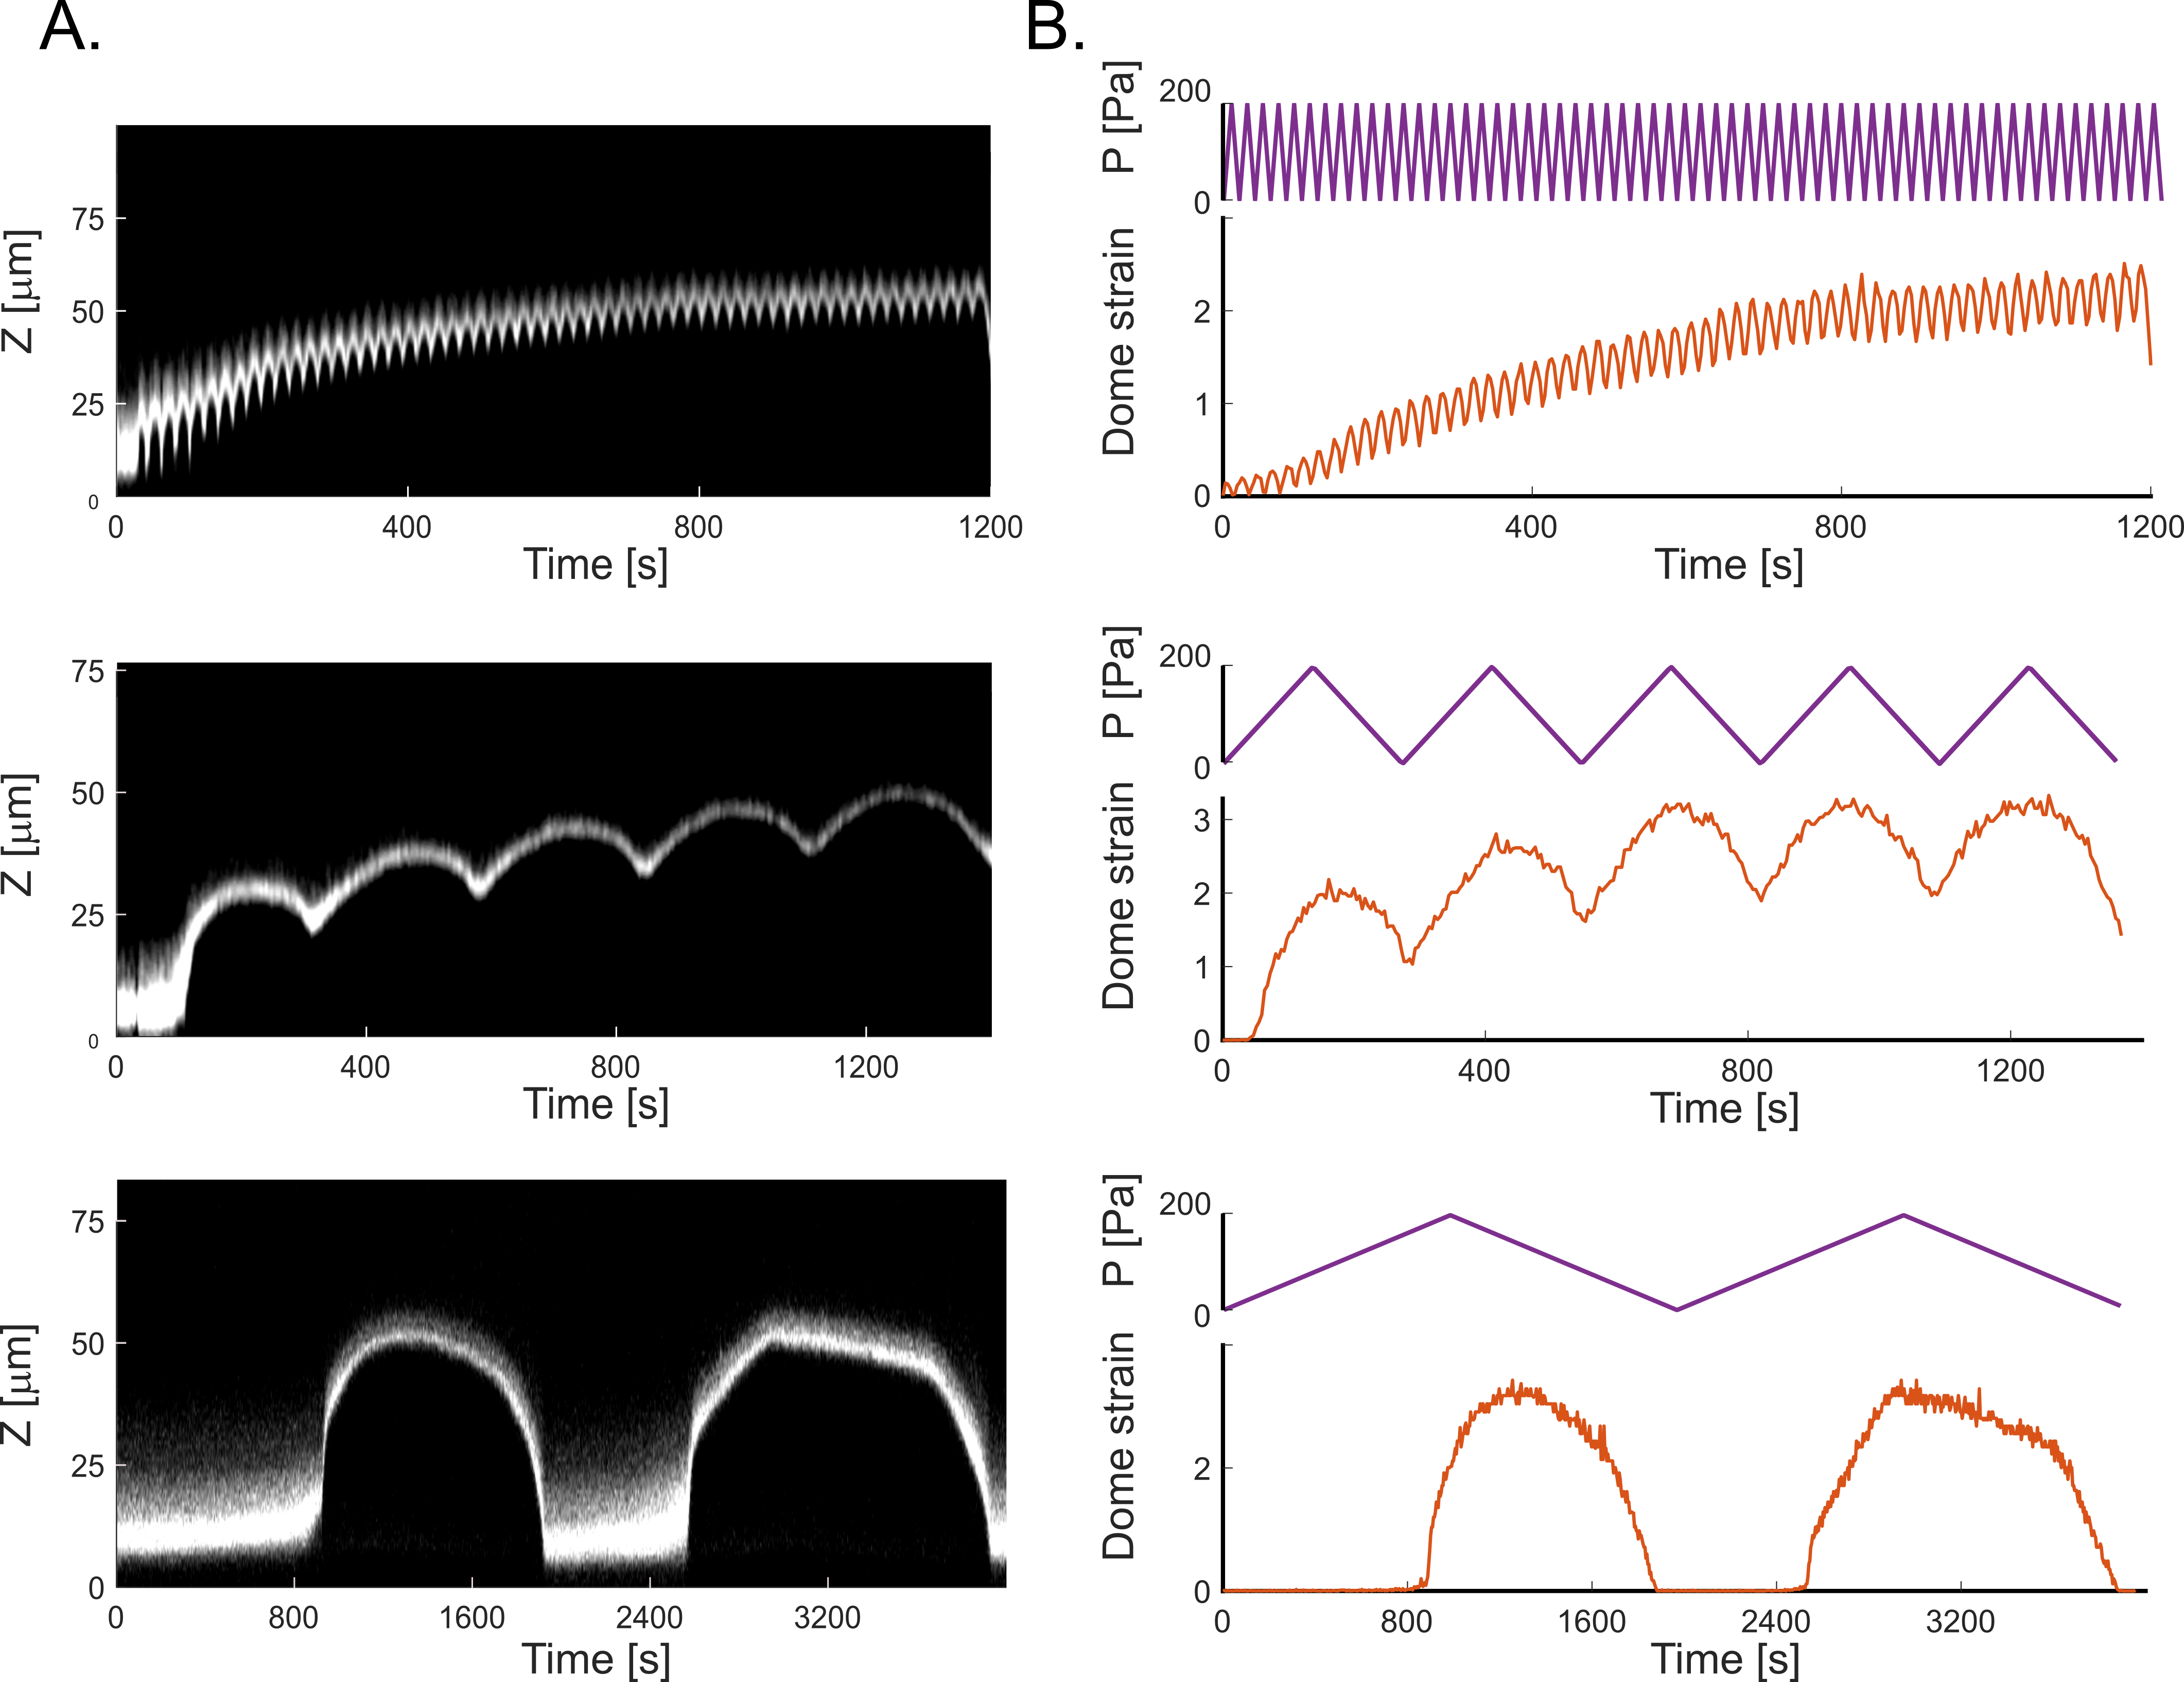
\includegraphics[width=\textwidth]{chap7_dynamic.png}
	\caption{\label{fig_7_6} \textbf{Dynamic response of Epithelia:} (A) The XZ plane images and kymographs of domes subjected to cyclic pressure between 0 to 200 Pa with rates of 20, 1.5, and 0.2 Pa/s The kymographs generated along the midsection of the domes indicated by yellow dotted lines. These indicate the evolution of height of the domes with respect to time. (B) The strain response of domes to cyclic pressure with different rates. Magenta represents pressure and red represents strain with respect to time. For A, B, n= 7 domes for 20 Pa/s, n = 8 for 1.5 Pa/s, and n = 7 for 0.2 Pa/s. 
	}
\end{figure}

\hypertarget{active-gel-tissue-model}{%
	\section{Active gel tissue model}\label{active-gel-tissue-model}}


We closely collaborated with Adam Ouzeri to develop a computational framework that incorporated the phenomenologies observed in our experiments. The existing literature on epithelial mechanics highlights the crucial role played by the viscoelasticity of the actin cortex in sustaining deformations over timescales spanning seconds to minutes \cite{kelkar2020,clement2017,khalilgharibi2019}. The theoretical framework developed herein serves as a bridge between active gel models of the actomyosin cortex and 3D vertex models at tissue scales \cite{ouzeri2023}. In this model, each cell is represented by an active gel surface that accounts for the physical attributes of the cortex, while a tissue is constructed from a collection of these active gel surfaces (as depicted in Fig \ref{fig_7_2}). The system's dynamics are formulated through a balance of diverse potentials representing various active internal or external forces and dissipation.

The framework accounts for the molecular dynamics of the actin filament network, myosin, and crosslinker proteins through four main components:

\begin{enumerate}
	\item \textbf{Cortical thickness:} The cell cortex is modeled as a hyperelastic membrane with cortical thickness ($\rho_R$). The deformation kinematics of this model is defined by mapping a cortical patch from a reference configuration ($\Gamma_0$) to a deformed configuration ($\Gamma$) with metric tensor \footnote{Metric  tensor, a mathematical object used in differential geometry, can be used to measure distances, angles, and volumes in curved spaces. Here, its measuring the cortical surface.} ($\mathbf{G_0}$) to ($\mathbf{g}$), respectively. To capture remodeling of cortex, the reference configuration has to be dynamic as well. Thus, there is a second reference configuration with a dynamic metric tensor ($\mathbf{G}$). The cortical thickness in the reference configuration changes with the mapping change represented by the Jacobian ($J_R$). This is expressed as 
	$$\rho_R(\mathbf{\xi}, t) = \rho(x,t)J_R(\mathbf{\xi},t).$$
	\item \textbf{Network elasticity:} This potential accounts for the free energy of the system undergoing deformation. The potential is dependent on the difference between in-plane strain ($\mathbf{C}$) and the metric ($\mathbf{G}$) written in the format of a hyperelastic potential ($W$). Using a Neo-Hookean elastic potential, $W$ depends on two Lamé parameters, ($\lambda$) and ($\mu$). This potential is expressed as $$\mathcal{F} = \int_{\Gamma_R} \rho_R \ W(\mathbf{C,G})dS_R.$$
	\item \textbf{Dissipation:} The actomyosin network remodels under tension, and the released elastic energy can be accounted for with a dissipation potential. The potential depends on a coefficient ($\eta$) equivalent to bulk viscosity, cortical thickness, and the rate of metric tensor given by ($\dot{\mathbf{G}}$). This potential is expressed as $$\mathcal{D} = \int_{\Gamma_R} \frac{\eta}{2}\ \rho_R \ \mathbf{\dot{G}}:\mathbf{\dot{G}} \ dS_R.$$
	\item \textbf{Active contractility:} The model is an active gel, and the active part is included through an active power potential that adds energy to the system. The potential is dependent on the cortical tension and the rate of deformation tensor. The cortical tension is an active tension component of the network that is proportional to cortical thickness. This potential is expressed as $\gamma(\rho) = \rho \xi$ and $$\mathcal{P} = \int_{\Gamma} \gamma : \mathbf{d} \ dS.$$
	
\end{enumerate}

Additionally, we account for turnover dynamics in the cortex through a mass balance law. Here, we assume that there is a steady-state cortical thickness, and the network is constantly polymerizing and depolymerizing with cytosolic components. This is expressed as $$\dot{\rho} + \rho \ tr(\mathbf{d}) = k_p\ C - k_d\ \rho.$$

The proposed governing equations are obtained by minimizing the Rayleighian, which is given as:

$$ \mathcal{R} = \frac{dF}{dt} - D + P + P_e .$$

Here, $P_e$ is an additional potential that accounts for external forces and tractions. The model assumes that the volume of the cell is conserved during deformation, and a mechanical barrier is introduced to prevent excessive strains beyond a threshold. This barrier is implemented by adding re-stiffening at large strains, which is necessary for physiological reasons, such as activation of intermediate filaments, cell crowding, or compression of the nucleus.

Overall, the system behaves like an active hyperelastic material at shorter timescales, while at longer timescales, it behaves like an active viscoelastic material.

The model was implemented to study dome system by creating a digital equivalent of the monolayer consisting of cell membranes. Non-adhesive regions were also included, which could be inflated into domes under pressure, similar to the experimental setup. Here after, we will refer to them as "digital domes" (see fig. \ref{fig_7_2}).


\begin{figure}[]
	\centering
	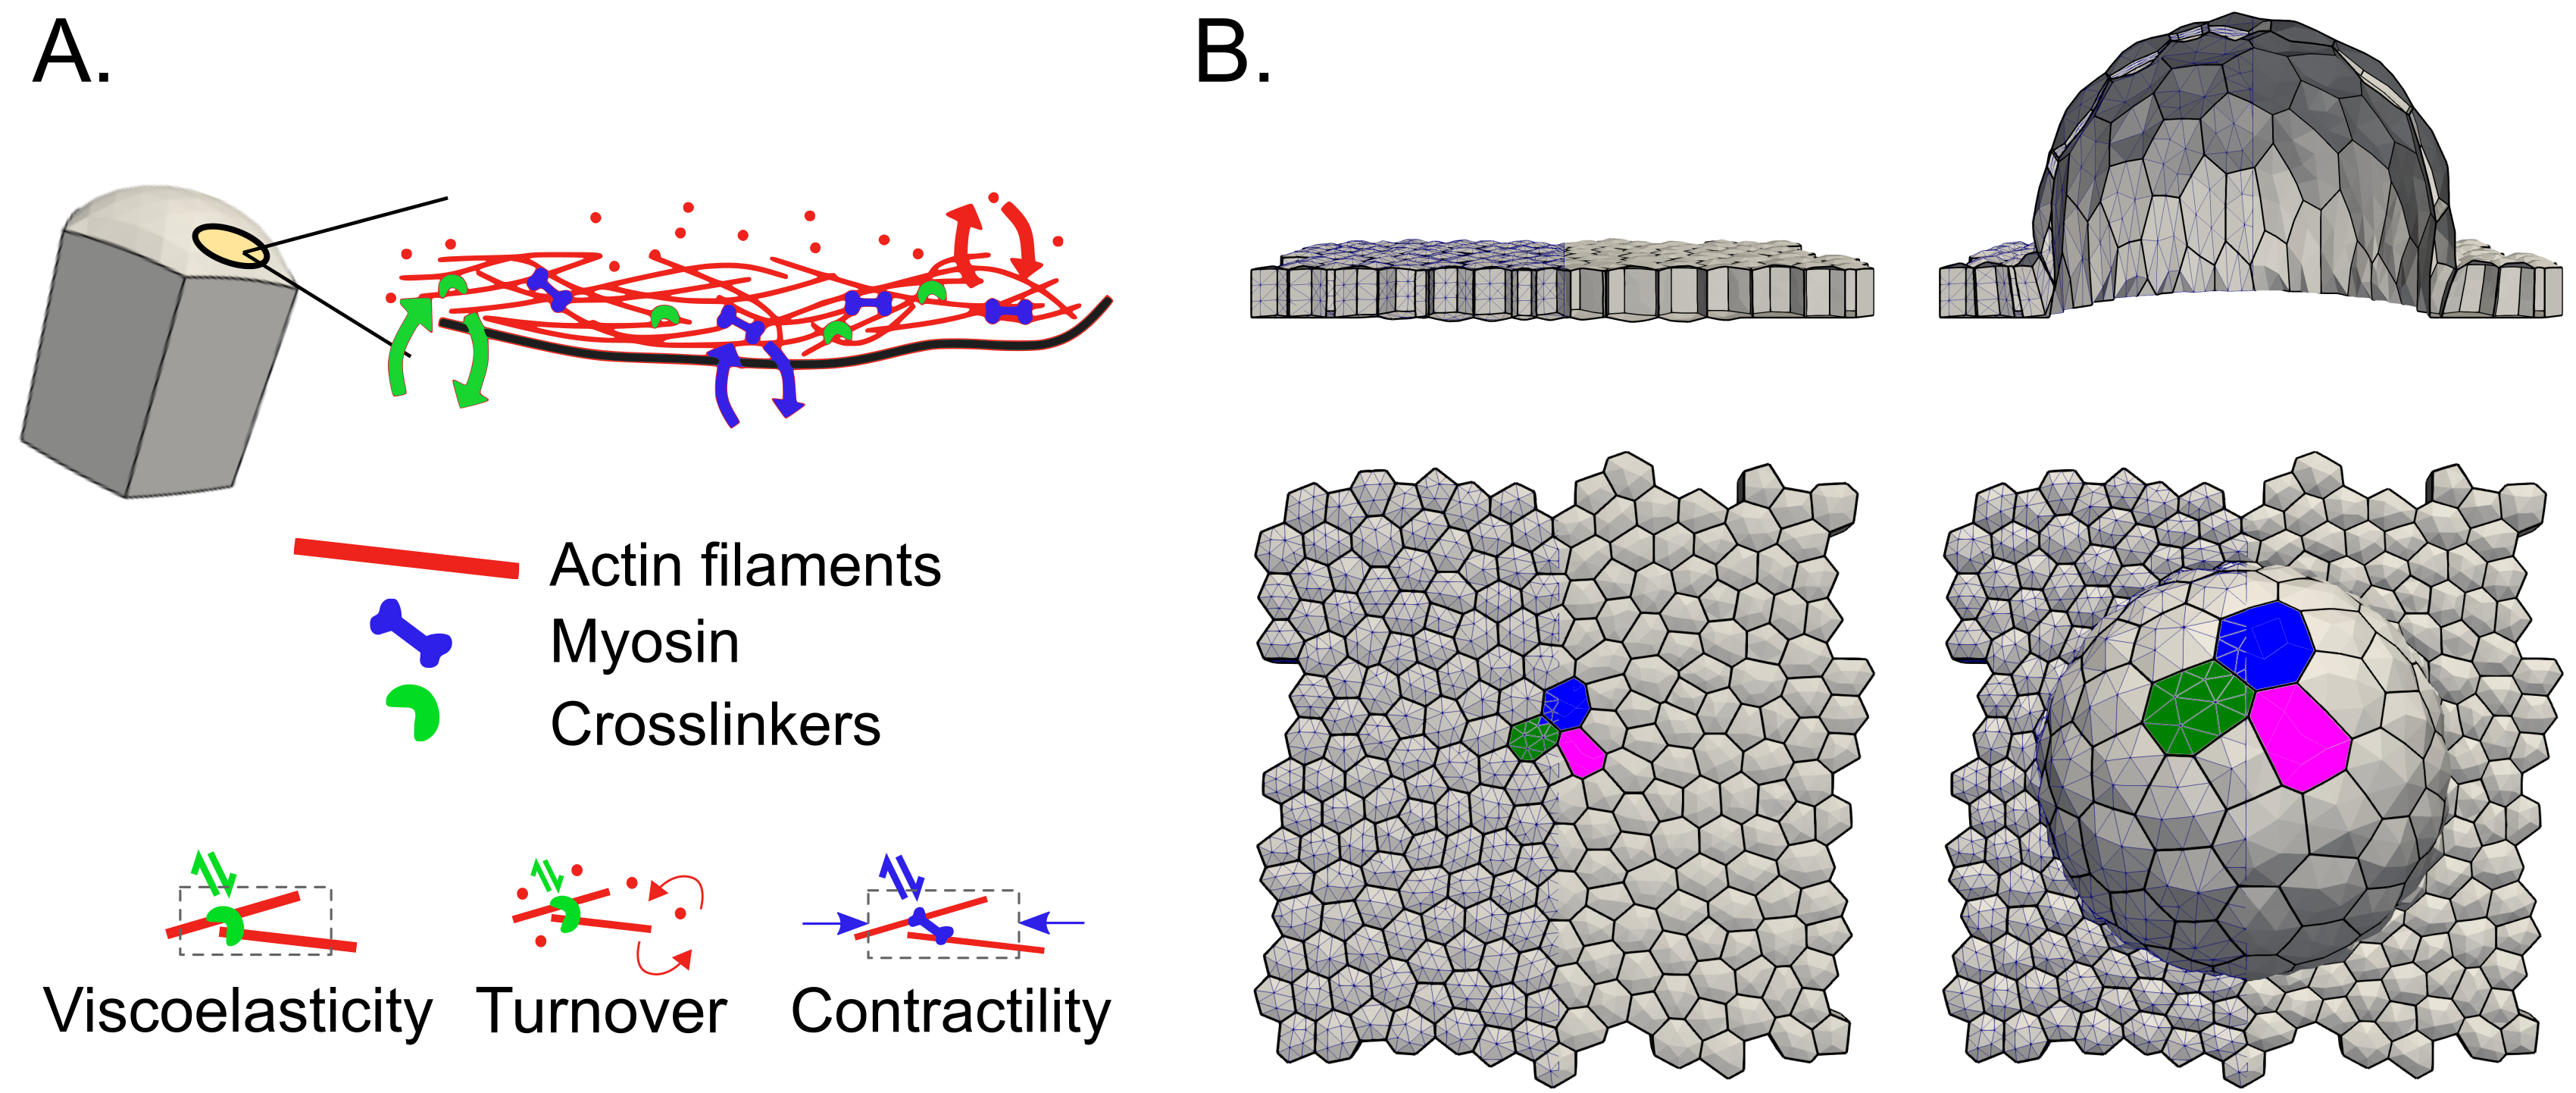
\includegraphics[width=\textwidth]{chap7_digitaldome.png}
	\caption{\label{fig_7_2} \textbf{Active gel tissue model}: (A) The cell is modeled as an active gel of cortex, which mainly comprises three aspects: viscoelasticity of the network, turnover dynamics, and active contractility. (B) These cells can be assembled into a tissue that can be used to perform in-silico experiments. An example of this is the digital dome being inflated, highlighting individual cells increasing their area.}
\end{figure}

\begin{center}
	
	\begin{mybox}{gray}{ \center{\label{A} \textbf{ Box A: Model summary}}}
		
	As the cortex undergoes stretching, we must consider its deformation through network elasticity. The cortical network is modeled as a hyperelastic membrane with a specific cortical thickness and the material parameter ($\lambda$).
	
	However, since the network relaxes due to turnover or contractility, we add a dissipative potential to account for the released elastic energy. This relaxation can be equated to viscous behavior, which can be represented by a viscosity coefficient ($\eta$) in the model. 
	
	To model active contractility, we incorporate an active power potential generated by the active tension ($\xi$) of the cortex. 
	
	Assumptions: 
	\begin{enumerate}
		\item The volume of the cell is conserved.
		\item The active tension is proportional to cortical thickness.
		\item There is a steady-state cortical thickness, and the network is continually turning over ($k_d$).
		\item To limit the strains, there is a strain stiffening mechanism which gets activated at high strains.		
	\end{enumerate}
	
	The model exhibits three timescales: 
	
	\begin{itemize}
		\item Turnover time $t_{to} = 1/k_d$
		\item Viscoelastic time $t_{ve} = \eta/\lambda$
		\item Viscoactive time $t_{va} = \eta/\xi$
	\end{itemize}
		
	\end{mybox}
	
\end{center}


\hypertarget{active-viscoelasticity-of-the-epithelia}{%
	\section{Active viscoelasticity of the
		epithelia}\label{active-viscoelasticity-of-the-epithelia}}
	
By conducting simulations that mirror the experimental conditions, we found that when digital domes were inflated with constant pressure, they reached a steady state while experiencing a reduction in cortical thickness as the cells stretched. Once the tissue tension was balanced by the applied pressure, the strain reached a stable point (see fig \ref{fig_7_7} A).

To obtain the constitutive relation, we inflated the digital dome with different pressures to obtain isobaric curves and steady state point. We also inflated a digital dome quasi-statically to assess the model’s robustness. We discovered that the constitutive relation obtained quasi-statically was consistent with the steady state locus in the isobarics (see fig \ref{fig_7_7} B). The constitutive curve exhibits similar characteristics to experiments, including clear re-stiffening at large strains, which we attribute to a barrier mechanism.

We interpreted these findings by using the concept of resting area, which refers to the area of a cell in a monolayer that is in a steady state. In the model, it is given by the metric tensor of dynamic reference configuration:

$$ A_{rest} = \int_{\Gamma_0} \sqrt{|\mathbf{G}|}dS_0, \text{ and } A_{actual} = \int_{\Gamma}dS. $$

When the tissue is perturbed from this state, the actual area can change faster than the resting area due to the viscoelastic behavior of the tissue. The cell dissipates elastic stresses at viscoelastic timescales through remodeling, eventually reaching a steady state. This effect of timescales is particularly evident in cyclic stretching experiments. When the cells are probed faster than viscoelastic timescales, they accumulate strains due to an inability to dissipate the elastic stress. In contrast, when stretching is slower, elastic stresses are dissipated with increasing area.

We observed that, for the slowest condition, the resting area in the digital dome almost overlapped with the actual area. This is because the pressure is changing very slowly at a rate of 0.2 Pa/s, allowing the cells sufficient time to remodel and dissipate elastic stresses. Viscoelastic and turnover timescales in simulations are around 10-30s, which means that over a period of 2000s, the dome stretches considerably and returns to original flat state.

However, when pressure is applied rapidly in cycles of 20 seconds, strains accumulate due to insufficient time for cells to dissipate stored elastic energy. The simulations show that the resting area marginally changes relative to the actual area. Notably, creep experiments, where tissue is stretched at constant tension, demonstrate strain accumulation at the visco-active timescale, where both contractility and viscosity play a role.

Interestingly, the simulations indicate that due to active viscoelasticity, there would be a lag between the peak of pressure and the peak of strain. This lag is clearly reflected in the comparison of resting area and actual area, where the delay decreases with increasing pressure rates. The slowest pressure rate results in the least amount of delay, while the fastest pressure rate results in the most delay. Although we can only experimentally observe this at moderate rates. The experimental data from faster cycles is too noisy to observe the lag.

To sum up, the digital dome model explains the material response of epithelial tissue depending on the rate at which pressure is applied. Slower rates allow for cell remodeling and dissipation of elastic stresses, while faster rates result in strain accumulation due to insufficient time for dissipation. This active viscoelastic behavior is the outcome of cortical remodeling.

\begin{figure}[t]
	\centering
	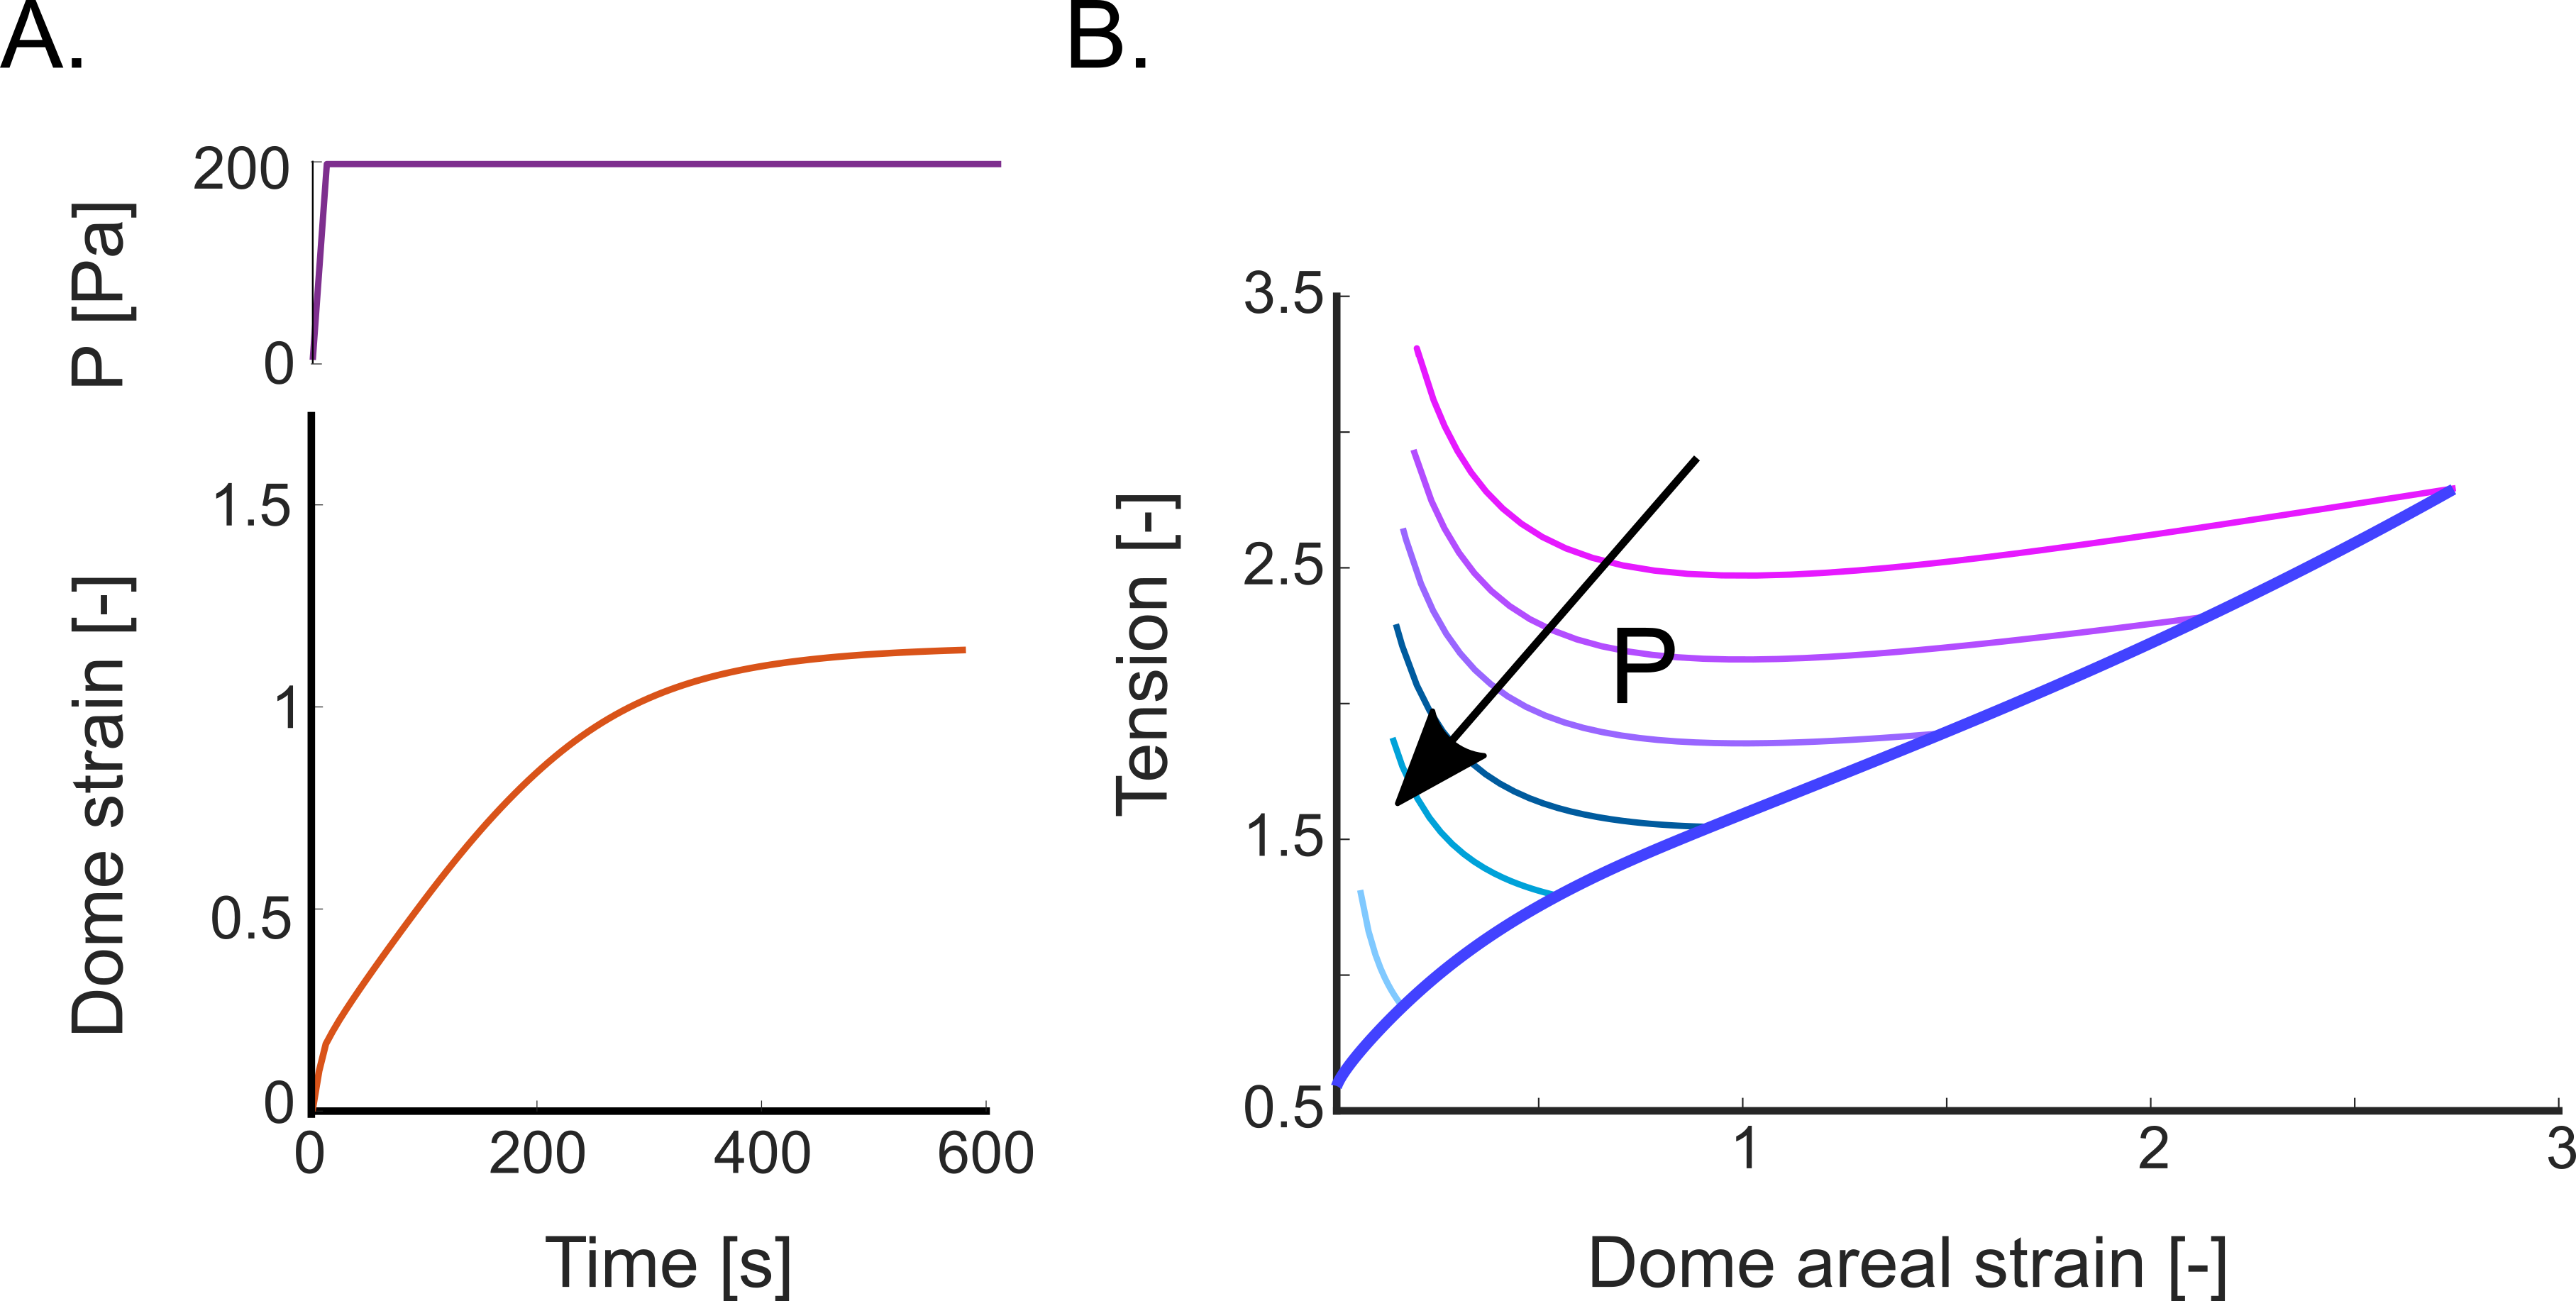
\includegraphics[width=\textwidth]{chap7_constitutivelawtwin.png}
	\caption{\label{fig_7_7} \textbf{Material response of the digital domes}: (A)  When subjected to constant pressure, as in experiments, the digital dome inflated and reached a steady state. (B)  These simulations also produced isobarics for different pressures, all leading to a steady state. Furthermore, subjecting it to a quasi-static increase in pressure produced a constitutive law (Navy blue curve) that can be mapped onto the locus of steady-state points.}
\end{figure}

\begin{figure}
	\centering
	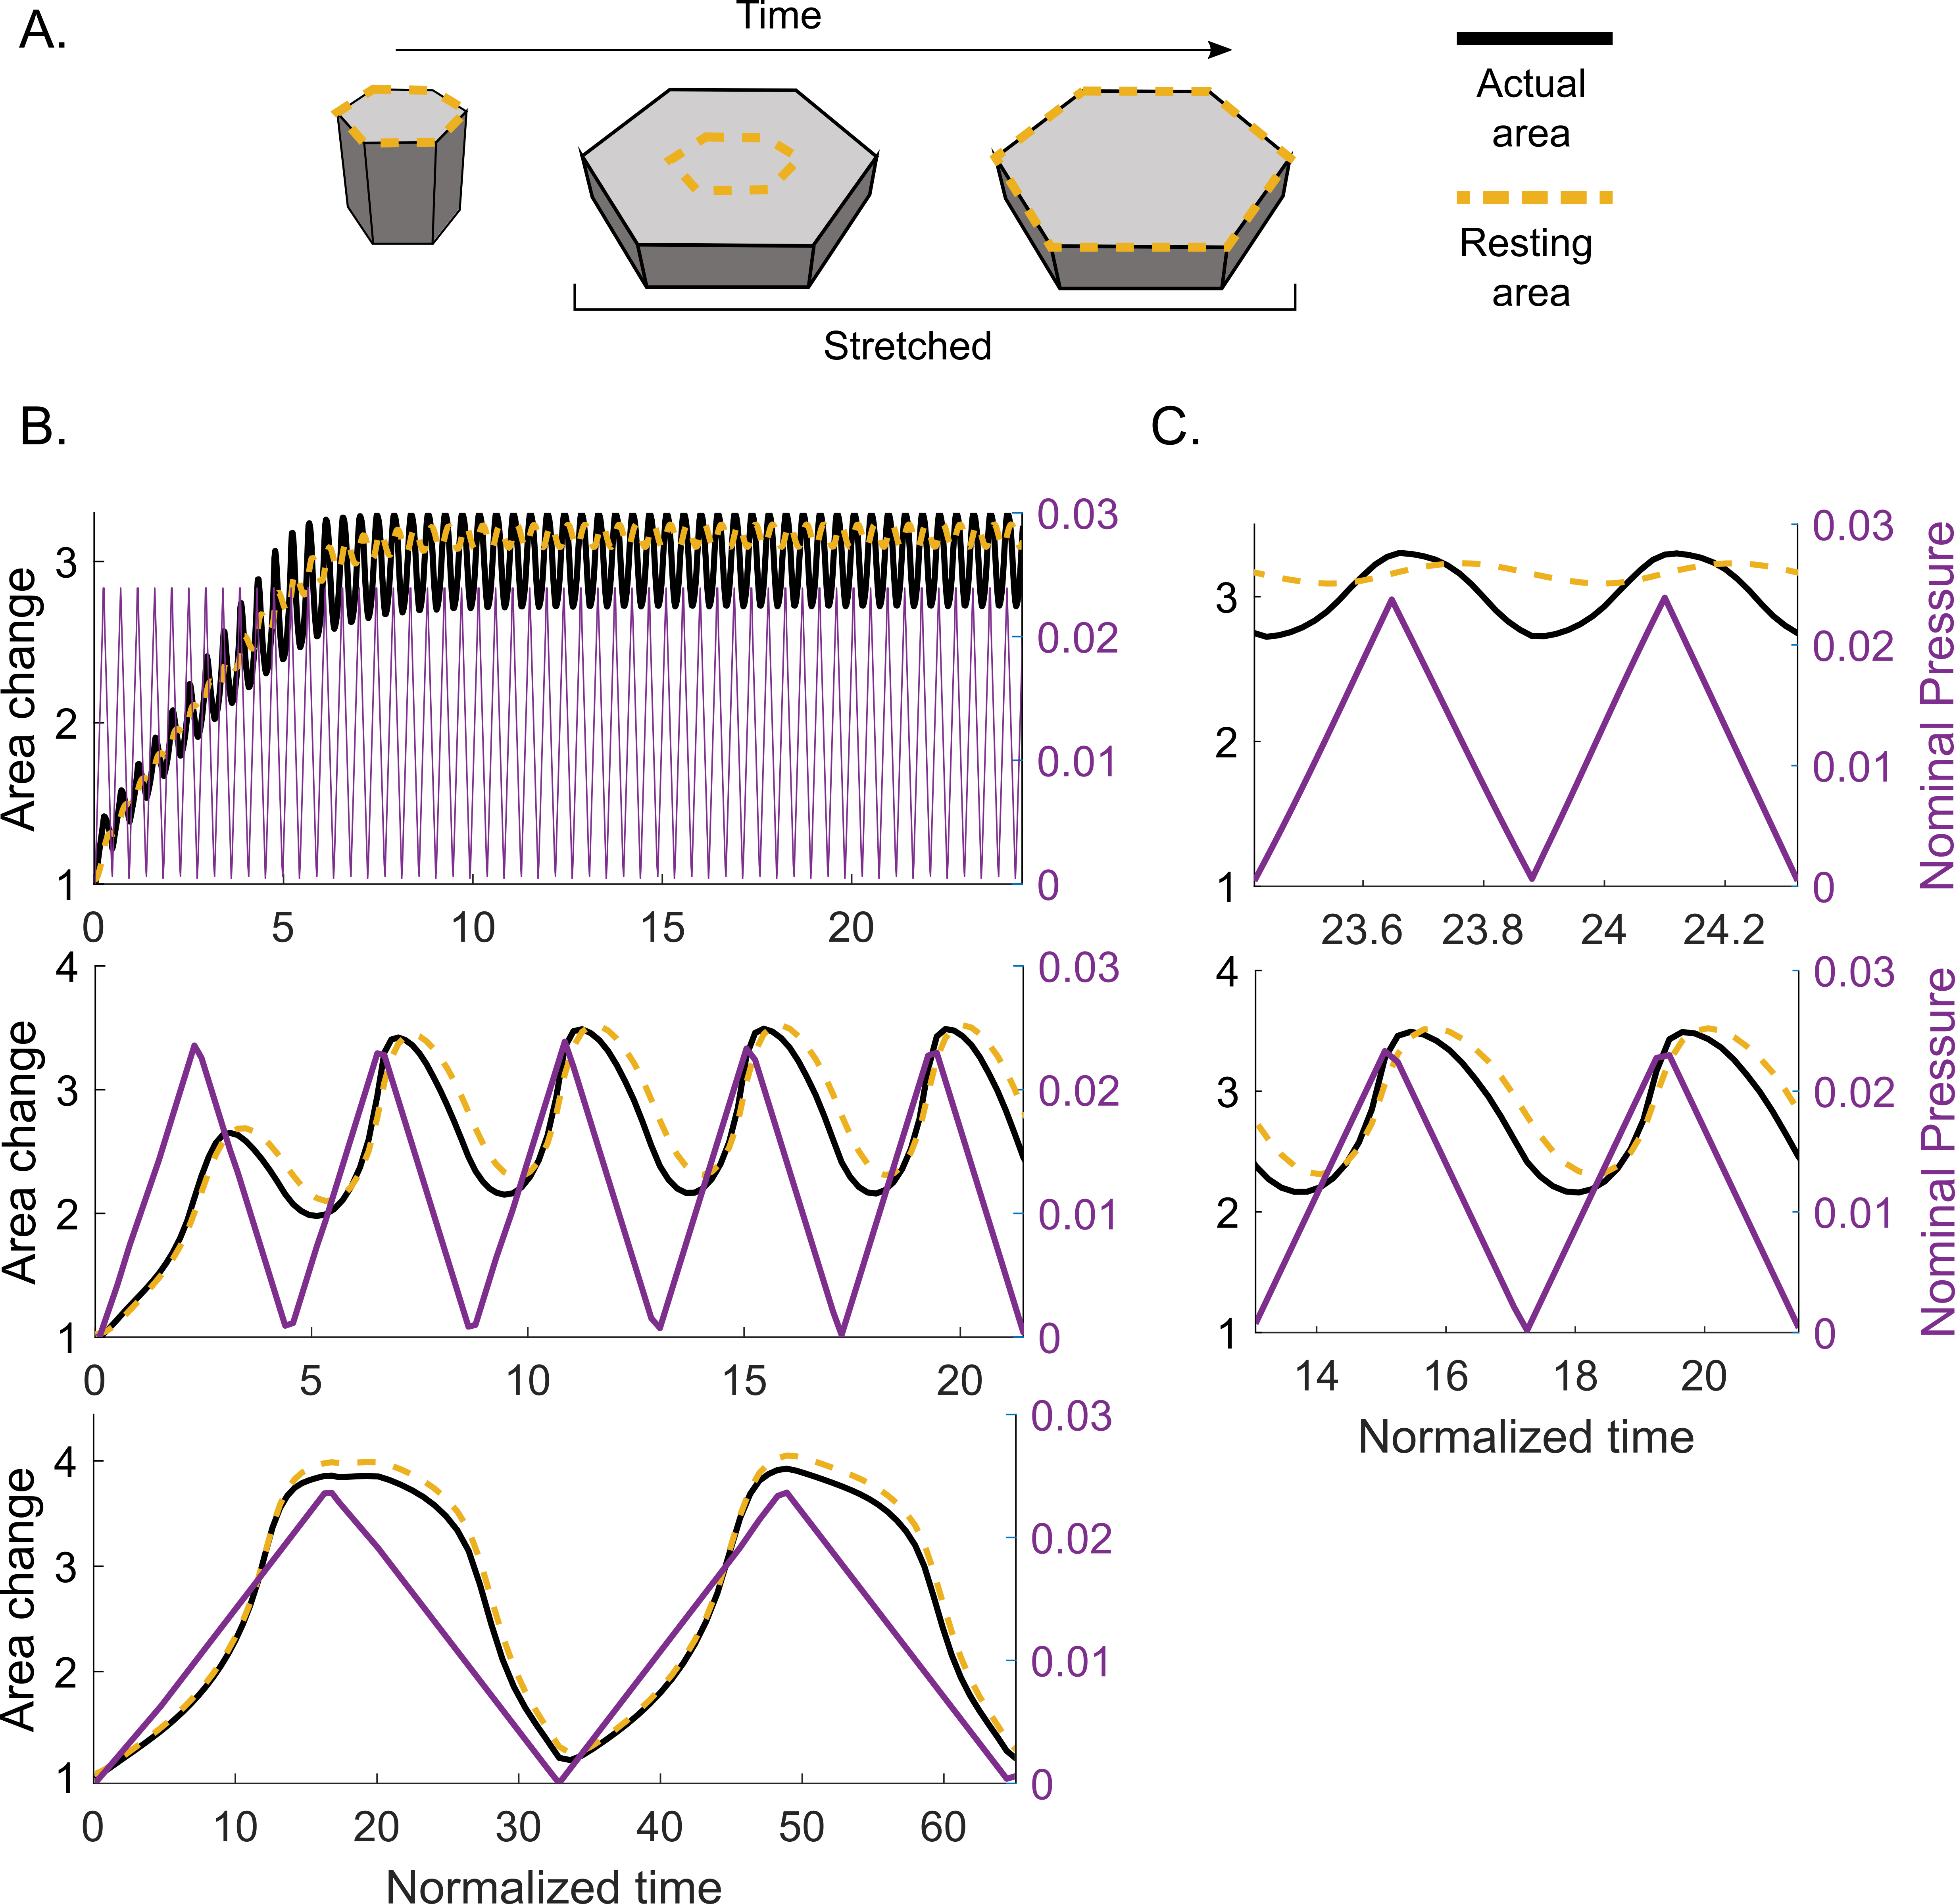
\includegraphics[width=\textwidth]{chap7_area.png}
	\caption{\label{fig_7_8} \textbf{Concept of resting area}: (A) Illustration of a resting and actual are of a cell in a monolayer during stretching. (B) Differences in results of resting and actual area when subjected to different rates of pressure. (C) Inset of the last two cycles.
	}
\end{figure}

\newpage
\hypertarget{summary}{%
	\section{Summary and Discussion}\label{summary}}

In this chapter, we investigated the mechanics of epithelial tissue by applying pressure at varying rates. Initially, we applied a constant pressure of 200Pa, which led to the dynamic inflation of domes and eventually reached a steady-state in strain. Due to the spherical geometry of the tissue, we observed a non-monotonous tension-strain curve in response to the constant pressure. However, we found that the true tension-strain curve exhibited increasing tension with respect to strains at lower values, but at higher strains, the tension appeared to be independent of the strains.

Furthermore, our measurements showed that the domes accumulated strain through the cycles when probed with fast-changing pressure and reached a steady-state in later cycles. However, when stretched slowly, the domes stretched to higher strains without accumulating strain at the end of the cycle.

To understand the behavior of epithelial tissue, we developed computational framework, which show that the response of the domes to cyclic pressure is dependent on active viscoelasticity.

The tissue stretches to balance the tissue tension with externally applied pressure timescale and reaches a steady-state strain by actively remodeling the cortex. Our digital dome studies indicated that different timescales play a role together in producing the tissue’s response to pressure. These timescales are the reflection of interplay between cortical turnover, crosslinkers, and network reorganization which allows for large deformations and rapid shape changes.

Our results can be interpreted using a multidimensional Maxwell model, which is a model that describes viscoelasticity. The classical Maxwell model consists of a spring and a dashpot, which represent the elastic and viscous elements, respectively. In our case, we can imagine a similar model with two branches: one branch includes a spring and a dashpot to represent the passive viscoelasticity, and a second branch includes an active spring to represent the active component  (see fig \ref{fig_7_9}). The active spring is always present, but if the stretching is done slowly, the dashpot would be driving the dominant mechanical response. Conversely, if the stretching is done rapidly, the elastic spring deformation would dominate. By separating the passive and active components, we can better understand how each contributes to the overall viscoelastic behavior and associated timescales.

Previous research has approached the system in a similar manner, where epithelial tissue was modeled using viscoelastic models of springs and dashpots. One particularly interesting model was developed by Khalilgharibi et. al., which characterizes the response of a suspended monolayer to stretch and demonstrates that the dynamics are similar to that of a single cell, due to the role of the actomyosin cortex \cite{khalilgharibi2019}. They used a model with two springs in parallel, one of which can change its resting length dynamically. This explains the relaxation of the monolayer, where the active contractility of the cortex changes the resting length of the active spring in the model, which closely relates to our "resting area" concept.

Another study found that viscoelastic dissipation could explain the shortening or elongation of cell junctions in drosophila embryos \cite{clement2017}. They demonstrated that the dissipation occurs at the minute timescale, at the same timescale as myosin pulses. It is also interesting that they found actin turnover plays a key role in this dissipation.

Applying tensions and strains to suspended cells in vitro is a challenging task, and it is important to note that adherent monolayers may exhibit different behaviors from suspended cells \cite{harris2012}. The tissue matrix provides additional stiffness and can alter the cytoskeletal structure of cells, which further complicates the understanding of cell mechanics \cite{humphrey2014, kechagia2019}. In this thesis, we focused on probing the response of suspended tissues at the short timescales (minutes), which is the timescale of acto-myosin network remodeling.

We did not observe any cellular rearrangement, extrusion, or division at this timescale in our system (with rare exceptions). Long-term experiments were not performed due to suspected involvement of other cytoskeletal components, such as intermediate filaments. In a study by Latorre et al., activation of intermediate filaments was observed in extremely stretched cells (>300\%), where they proposed that this is caused re-stiffening and prevented the cells from stretching too much  \cite{latorre2018}. This motivated the strain limiting mechanism imposed in our model. However, in our experiments, we did not observe any indication of superelasticity, as all cells were super-stretched at the same time. This might be due to the relatively shorter timescales in our experiments compared to long term quasi-static deformation of spontaneous domes.

\textbf{About strain stiffning and results of \cite{duque2023}. About racheting of contractile force \cite{clement2017, mason2011} and strain accumulation or creep}

In the next chapter, we will endeavor to apply our understanding of viscoelasticity to generate radical transformation of domes into various structures.

\begin{figure}
	\centering
	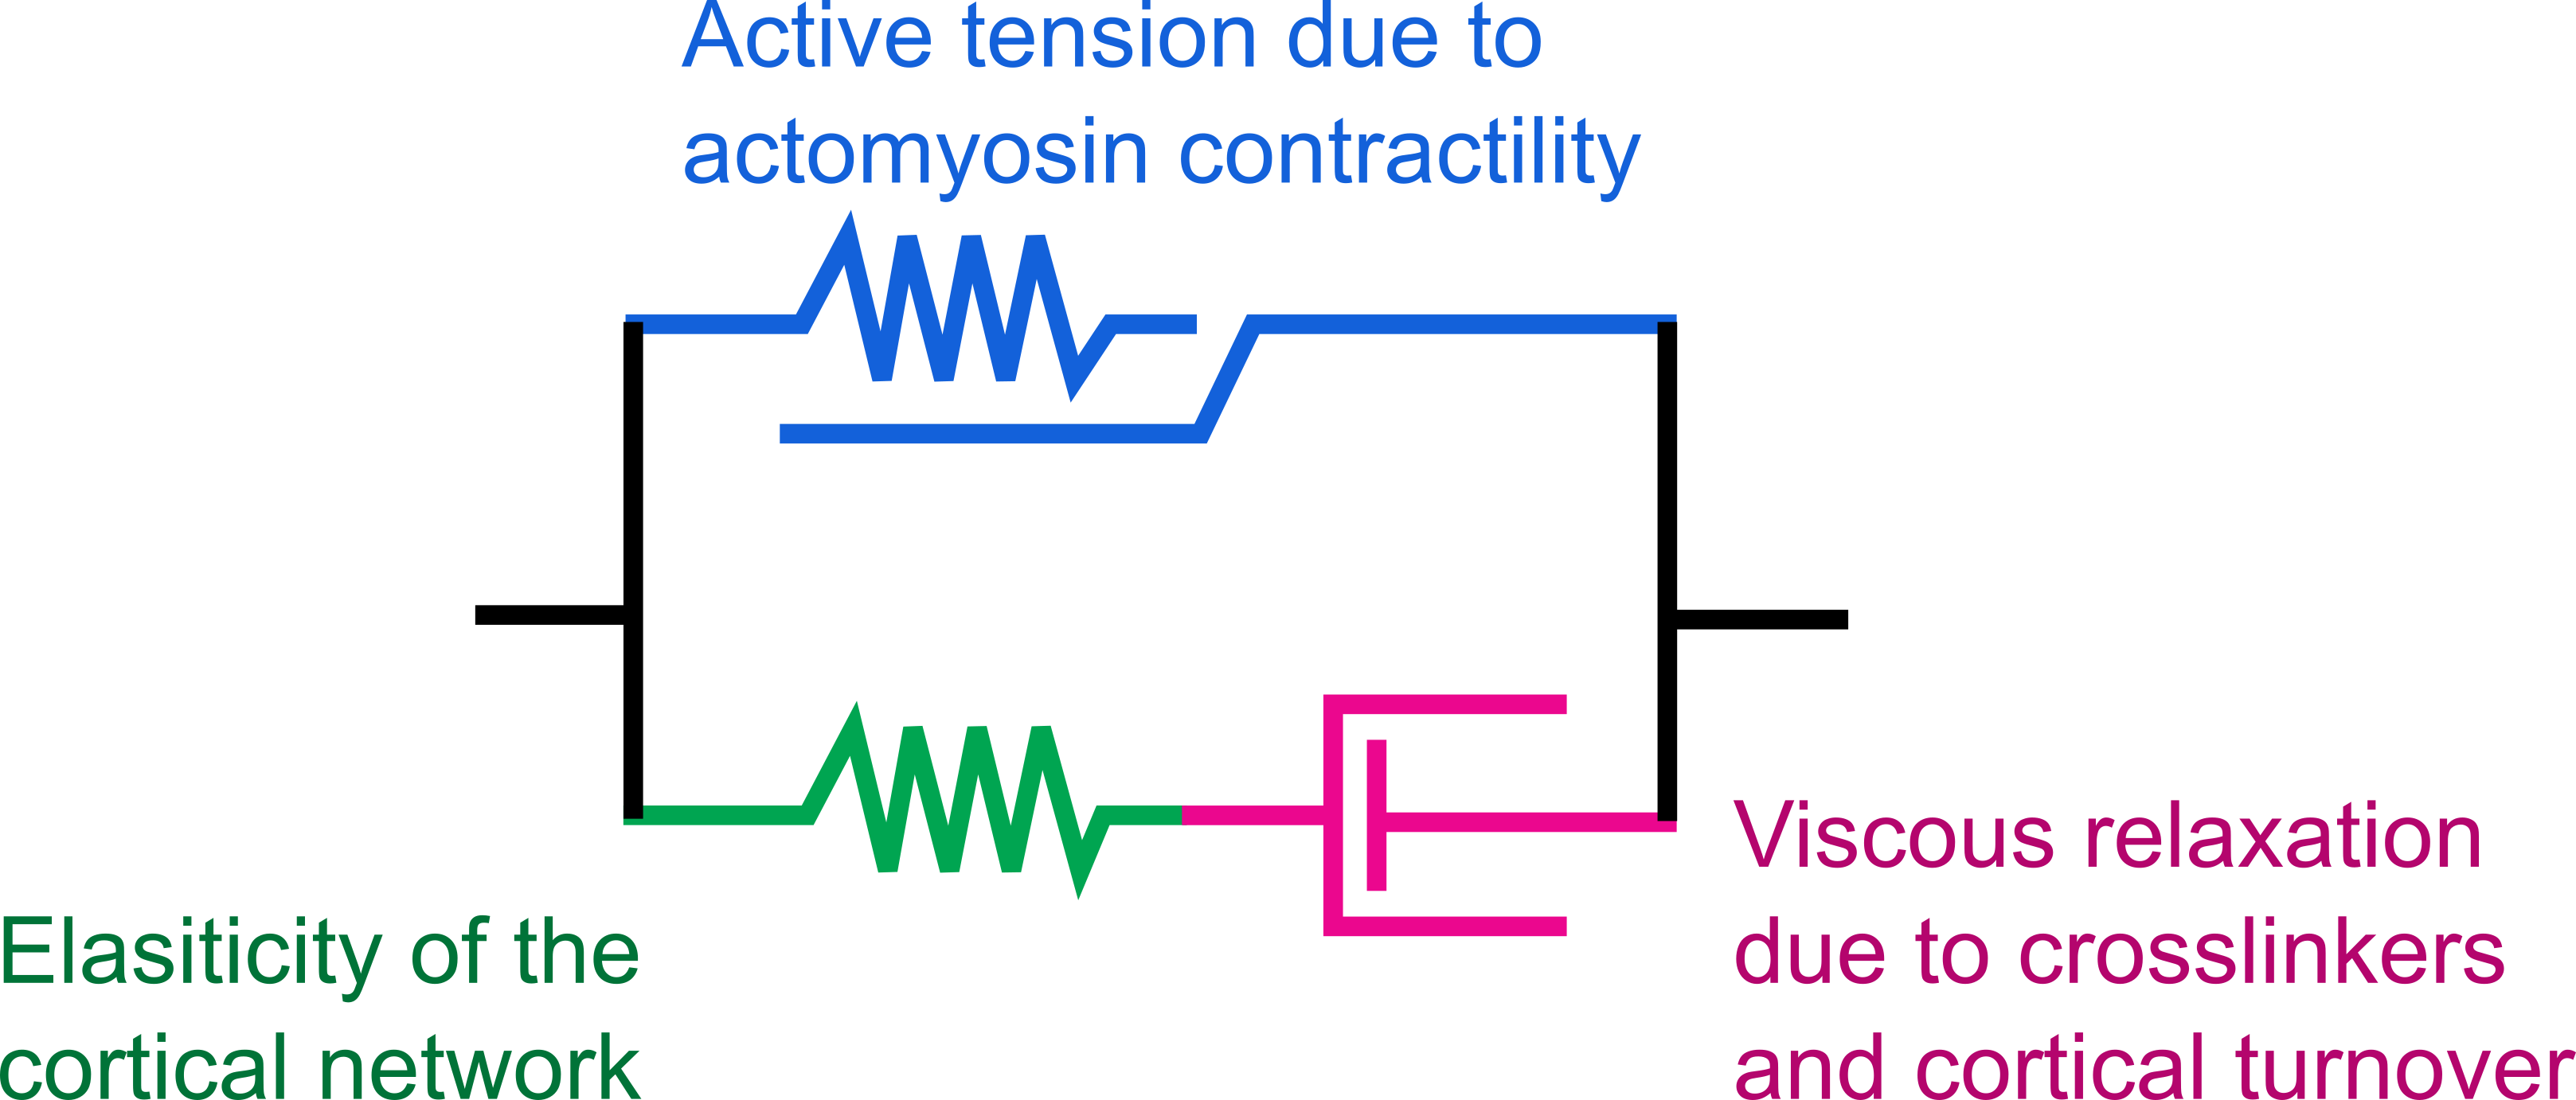
\includegraphics[width=0.75\textwidth]{chap7_maxwell.png}
	\caption{\label{fig_7_9} \textbf{Representational viscoelasticity model}: The model can be understood using a spring and dashpot analogy with two branches: The first branch is an active spring representing the contractile forces applied by the actomyosin cortex. The second branch has two components, one for the elasticity of the network and the second for the viscous relaxation that occurs due to turnover of the network.
	}
\end{figure}